\chapter{Some Elementary Statistical Inferences}\label{chap:elementary-statistical-inferences}

\section*{Chapter 4 Overview}

在前三章中，我们建立了描述随机变量和概率分布的理论框架。现在我们面临一个根本性问题：

\begin{center}
\textit{给定观测数据，如何推断产生这些数据的底层分布？}
\end{center}

这个问题——从已知数据推断未知规律——正是统计学的核心任务。正如 Fisher 在 1922 年的经典论文中所强调的，统计推断的本质是在不确定性下做出明智决策。

本章介绍三种主要的推断工具：
\begin{itemize}
\item \textbf{点估计}（Point Estimation）：用单一数值估计未知参数
\item \textbf{置信区间}（Confidence Intervals）：参数的合理取值范围，而非点估计的单一数值
\item \textbf{假设检验}（Hypothesis Testing）：评估关于总体的声明是否获得数据支持
\end{itemize}

这三种工具相互关联：点估计给出参数的最佳猜测，置信区间度量这个猜测的精度，而假设检验则让我们能够验证关于总体的具体声明。

\textbf{本章路线图}：抽样与统计量 $\to$ 点估计（MLE）$\to$ 置信区间 $\to$ 假设检验 $\to$ 卡方检验 $\to$ 蒙特卡洛 $\to$ Bootstrap

\section{4.1 Sampling and Statistics}\label{sec:4.1}

\subsection{从总体到样本}

在典型的统计问题中，我们关心某个随机变量 $X$，但其 pdf $f(x)$ 或 pmf $p(x)$ 未知。这种未知性可以分为两类：

\begin{enumerate}
\item $f(x)$ 或 $p(x)$ 的形式完全未知
\item 分布的形式已知，但包含未知参数 $\theta$（$\theta$ 可以是向量）
\end{enumerate}\footnote{第一种情况属于非参数方法（Chapter 10 深入讨论），第二种情况是本章的核心内容。见附录 \cref{sec:qa-parametric-vs-nonparametric}。}

\textbf{本章聚焦第二类}——这正是统计学中最常见的场景。我们已知数据的分布类型，只是不知道具体的参数值。几个典型例子：

\begin{itemize}
\item[(a)] $X \sim \mathrm{Exp}(\theta)$，$\theta$ 未知——指数分布常用于描述等待时间
\item[(b)] $X \sim \mathrm{Binomial}(n,p)$，$p$ 未知——二项分布描述 $n$ 次试验中的成功次数
\item[(c)] $X \sim \Gamma(\alpha,\beta)$，$\alpha$ 和 $\beta$ 均未知——Gamma 分布广泛出现于保险和排队论
\item[(d)] $X \sim N(\mu,\sigma^2)$，$\mu$ 和 $\sigma^2$ 均未知——正态分布是统计学的心脏
\end{itemize}

我们用 $f(x;\theta)$ 或 $p(x;\theta)$ 表示含参分布，其中 $\theta \in \Omega$，$\Omega$ 是参数空间（所有可能的 $\theta$ 组成的集合）。

\subsection{随机样本}

\textbf{为什么要强调"随机"抽取？} 因为只有随机抽样才能保证样本具有代表性——每个个体被选中的概率相等，这样样本才能"代表"总体。

从总体中抽取样本，样本观测值与 $X$ 同分布。记为随机变量 $X_1, X_2, \ldots, X_n$，其中 $n$ 是样本量。抽到具体数值后记为 $x_1, x_2, \ldots, x_n$。

若 $X_1, \ldots, X_n$ 相互独立且同分布，则称它们为来自该共同分布的\textbf{随机样本（random sample）}。

\begin{definition}[随机样本]\label{def:random-sample-ch4}
如果随机变量 $X_1, X_2, \ldots, X_n$ 独立同分布（iid），则称这些随机变量构成来自该共同分布的容量为 $n$ 的随机样本。
\end{definition}

从这个定义出发，样本的联合 pdf/pmf 为
\[
f(x_1, \ldots, x_n; \theta) = \prod_{i=1}^n f(x_i; \theta),
\]
这正是后续推导似然函数的基础。

\subsection{统计量}

我们已经学会了如何描述单个随机变量，现在面临一个新问题：\textbf{如何从样本中提取信息？}

设 $T = T(X_1, X_2, \ldots, X_n)$ 是样本的函数。则称 $T$ 为一个\textbf{统计量（statistic）}。

统计量的关键特征在于：\textbf{不依赖任何未知参数}。换言之，统计量只基于观测数据进行计算，不涉及任何未知数。一旦样本被观测，$t = T(x_1, \ldots, x_n)$ 称为 $T$ 的实现值。

\section{4.2 Point Estimation}\label{sec:4.2}

点估计提供一个单一数值（记作 $\widehat{\theta}$）作为未知参数 $\theta$ 的估计。但这里立刻产生一个问题：如何找到"好"的估计量？

\subsection{无偏性}

\textbf{我们希望估计量具有什么性质？} 最基本的要求是无偏性——如果反复抽样，估计量的平均值应该等于真实参数值。

\begin{definition}[无偏估计量]\label{def:unbiased-estimator}
设 $X_1, \ldots, X_n$ 是来自分布 $f(x;\theta)$ 的样本，$\theta \in \Omega$。设 $T = T(X_1, \ldots, X_n)$ 是统计量。若
\[
\mathbb{E}(T) = \theta,
\]
则称 $T$ 是 $\theta$ 的\textbf{无偏估计量（unbiased estimator）}。
\end{definition}

若 $\mathbb{E}(T) \neq \theta$，则称 $\mathrm{Bias}(T) = \mathbb{E}(T) - \theta$ 为偏差。无偏性保证估计量没有系统性偏差——既不高估也不低估。

\textbf{注意}：无偏性并不保证估计量"最好"。例如，样本方差 $S^2$ 是无偏的，但 $n^{-1}\sum(X_i - \bar{X})^2$ 是有偏的。这引发了一个自然的问题：能否找到一个统一的、"最优"的估计原则？\footnote{问：为什么要举这个例子？它在整个章节中起什么作用？见附录 \cref{sec:qa-unbiasedness-transition}。}

\subsection{最大似然估计（MLE）}

\textbf{为什么需要似然函数？} 样本来自参数 $\theta$ 的分布 $f(x;\theta)$。给定 $\theta$ 时，观察到当前数据 $\mathbf{x} = (x_1, \ldots, x_n)$ 的概率（密度）为 $f(\mathbf{x}; \theta)$。似然函数正是这个想法的数学表达——它衡量在给定 $\theta$ 时，观察到当前数据的"可能性"。\footnote{在贝叶斯统计中，似然函数与先验分布结合通过贝叶斯定理产生后验分布。见附录 \cref{sec:qa-bayesian-prior-examples}。}

\begin{definition}[似然函数]\label{def:likelihood-function-ch4}
设 $X_1, \ldots, X_n$ 是来自 $f(x;\theta)$ 的随机样本。则
\[
L(\theta) = L(\theta; x_1, \ldots, x_n) = \prod_{i=1}^n f(x_i; \theta)
\]
称为该随机样本的\textbf{似然函数（likelihood function）}。
\end{definition}

\textbf{核心思想}：如果 $\theta$ 是真实参数，那么它应该使得观察到的数据具有较高的"可能性"。因此，我们选择使 $L(\theta)$ 最大化的 $\widehat{\theta}$——这正是最大似然估计量的定义。

最大似然估计量（MLE）：
\[
\widehat{\theta} = \underset{\theta}{\operatorname{argmax}} \, L(\theta).
\tag{4.2.1}\label{eq:mle-definition}\]
\]

在实际计算中，通常使用对数似然 $l(\theta) = \log L(\theta)$，因为 $\log$ 是严格递增函数，最大化 $l(\theta)$ 等价于最大化 $L(\theta)$。在正则条件下，$\widehat{\theta}$ 满足
\[
\frac{\partial l(\theta)}{\partial \theta} = 0. \tag{4.2.2}\label{eq:mle-score-equation}\]
\]

这个方程称为\textbf{似然方程（score equation）}。\footnote{通用推导框架见附录 \cref{sec:derivation-mle}。}

\begin{example}[指数分布的 MLE]\label{ex:exponential-mle-ch4}
设 $X_1, \ldots, X_n \sim \mathrm{Exp}(\theta)$，pdf 为 $f(x) = \theta^{-1}\exp\{-x/\theta\}$，$x>0$。

对数似然为
\[
l(\theta) = -n\log\theta - \frac{1}{\theta}\sum_{i=1}^n x_i.
\]

令导数为零，解得 $\widehat{\theta} = \bar{x}$。由于 $\mathbb{E}(X) = \theta$，故 $\widehat{\theta} = \bar{X}$ 也是无偏估计。\footnote{详细推导见附录 \cref{sec:derivation-exponential-mle}。}
\end{example}

\begin{example}[二项分布的 MLE]\label{ex:binomial-mle-ch4}
设 $X \sim \mathrm{Bernoulli}(\theta)$，$p(x;\theta) = \theta^x(1-\theta)^{1-x}$，$x=0,1$。

对于随机样本，似然函数为
\[
L(\theta) = \theta^{\sum x_i}(1-\theta)^{n-\sum x_i}.
\]

对数似然求导并令为零，解得 $\widehat{\theta} = \bar{x}$。由于 $\mathbb{E}(X) = \theta$，故 $\widehat{\theta} = \bar{X}$ 是无偏的。\footnote{详细推导见附录 \cref{sec:derivation-binomial-mle}。}
\end{example}

\begin{example}[正态分布的 MLE]\label{ex:normal-mle-ch4}
设 $X_1, \ldots, X_n \sim N(\mu, \sigma^2)$，参数向量为 $\boldsymbol{\theta} = (\mu, \sigma)$。

对数似然为
\[
l(\mu, \sigma) = -\frac{n}{2}\log 2\pi - n\log\sigma - \frac{1}{2}\sum_{i=1}^n\left(\frac{x_i - \mu}{\sigma}\right)^2.
\tag{4.2.3}\label{eq:normal-log-likelihood}\]
\]

对 $\mu$ 和 $\sigma$ 分别求偏导并令为零，解得
\[
\widehat{\mu} = \bar{X}, \tag{4.2.4}\label{eq:mle-normal-mu}\]
\]
\[
\widehat{\sigma}^2 = \frac{1}{n}\sum_{i=1}^n (X_i - \bar{X})^2. \tag{4.2.5}\label{eq:mle-normal-sigma}\]
\]

\textbf{一个重要发现}：$\widehat{\mu} = \bar{X}$ 是无偏的（$\mathbb{E}(\bar{X}) = \mu$），但 $\widehat{\sigma}^2$ 是\textbf{有偏}的——
\[
\mathbb{E}(\widehat{\sigma}^2) = \frac{n-1}{n}\sigma^2,
\]
而样本方差 $S^2 = \frac{1}{n-1}\sum_{i=1}^n (X_i - \bar{X})^2$ 是无偏的（$\mathbb{E}(S^2) = \sigma^2$）。这说明 MLE 有时并非无偏——无偏性和最大似然是两种不同的估计原则。\footnote{详细推导见附录 \cref{sec:derivation-normal-mle}。}
\end{example}

MLE 的吸引力来自其渐近理论：在温和条件下，MLE 是渐近正态的、渐近有效的，且具有最优性。这些性质使 MLE 成为现代统计推断的基石。

\section{4.3 Confidence Intervals}\label{sec:4.3}

点估计给出一个数值，但它没有告诉我们这个估计有多"可靠"。置信区间通过提供参数的取值范围来解决这个问题。

\textbf{一个直观的类比}：如果点估计是"我认为明天的温度是 22 度"，那么置信区间就是"我认为温度在 18 到 26 度之间"。后者不仅给出估计，还表达了不确定性。

\begin{definition}[置信区间]\label{def:confidence-interval-ch4}
设 $L = g_1(X_1, \ldots, X_n)$ 和 $U = g_2(X_1, \ldots, X_n)$ 是两个统计量。若对所有 $\theta \in \Omega$，
\[
\mathbb{P}_\theta(L \leq \theta \leq U) = 1 - \alpha,
\]
则称随机区间 $[L, U]$ 为 $\theta$ 的 $100(1-\alpha)\%$ \textbf{置信区间（confidence interval）}。
\end{definition}

\textbf{正确理解}：不是说"$\theta$ 以 $1-\alpha$ 概率落在区间内"（$\theta$ 是固定常数，没有随机性），而是说"如果重复抽样 $100(1-\alpha)\%$ 的区间会包含 $\theta$"。这称为置信区间的频率学派解释。\footnote{问：很多初学者把置信区间的定义 $\mathbb{P}_\theta(L \leq \theta \leq U) = 1 - \alpha$ 误解为"$\theta$ 有 $1-\alpha$ 的概率落在区间 $[L, U]$ 中"。这两种解释有什么区别？见附录 \cref{sec:qa-confidence-interval-frequentist}。}

\textbf{构造置信区间的关键}是找到枢轴量（pivot）——一个其分布不依赖于未知参数的函数。\footnote{枢轴量的构造方法及推导见附录 \cref{sec:derivation-confidence-interval}。}

\subsection{正态均值的置信区间}

\begin{example}[已知方差]\label{ex:ci-normal-known}
设 $X_1, \ldots, X_n \sim N(\mu, \sigma^2)$，$\sigma^2$ 已知。则 $\mu$ 的 $100(1-\alpha)\%$ 置信区间为
\[
\left[ \bar{X} - z_{\alpha/2}\frac{\sigma}{\sqrt{n}},\quad \bar{X} + z_{\alpha/2}\frac{\sigma}{\sqrt{n}} \right],
\tag{4.3.1}\label{eq:ci-normal-known}\]
\]
其中 $z_{\alpha/2}$ 满足 $\Phi(z_{\alpha/2}) = 1 - \alpha/2$。

\textbf{直觉理解}：区间宽度 $\propto \sigma/\sqrt{n}$——样本量越大，估计越精确。这与大数定律的直觉一致：更多信息带来更精确的估计。\footnote{详细推导见附录 \cref{sec:derivation-normal-ci-known}。}
\end{example}

\begin{example}[未知方差]\label{ex:ci-normal-unknown}
设 $X_1, \ldots, X_n \sim N(\mu, \sigma^2)$，$\sigma^2$ 未知。用 $S^2$ 替代 $\sigma^2$，则
\[
\frac{\bar{X} - \mu}{S/\sqrt{n}} \sim t_{n-1},
\tag{4.3.2}\label{eq:t-statistic}\]
\]
故 $\mu$ 的 $100(1-\alpha)\%$ 置信区间为
\[
\left[ \bar{X} - t_{\alpha/2,n-1}\frac{S}{\sqrt{n}},\quad \bar{X} + t_{\alpha/2,n-1}\frac{S}{\sqrt{n}} \right].
\tag{4.3.3}\label{eq:ci-normal-unknown}\]
\]

\textbf{用 $t$ 分布替代正态分布}：当方差未知时，我们用样本标准差 $S$ 替代总体标准差 $\sigma$。这引入了额外的随机性，导致分布从正态变为 $t$ 分布。$t$ 分布比正态分布更"重尾"，反映了未知方差带来的不确定性。\footnote{详细推导见附录 \cref{sec:derivation-normal-ci-unknown}。}
\end{example}

\begin{theorem}[方差置信区间]\label{th:ci-variance-ch4}
设 $X_1, \ldots, X_n \sim N(\mu, \sigma^2)$。则 $\sigma^2$ 的 $100(1-\alpha)\%$ 置信区间为
\[
\left[ \frac{(n-1)S^2}{\chi^2_{\alpha/2,n-1}},\quad \frac{(n-1)S^2}{\chi^2_{1-\alpha/2,n-1}} \right].
\tag{4.3.4}\label{eq:ci-variance}\]
\]
其中 $\chi^2_{p, k}$ 是 $\chi^2(k)$ 分布的上侧 $p$ 分位数。\footnote{详细推导见附录 \cref{sec:derivation-variance-ci}。}
\end{theorem}

\begin{figure}[H]
\centering
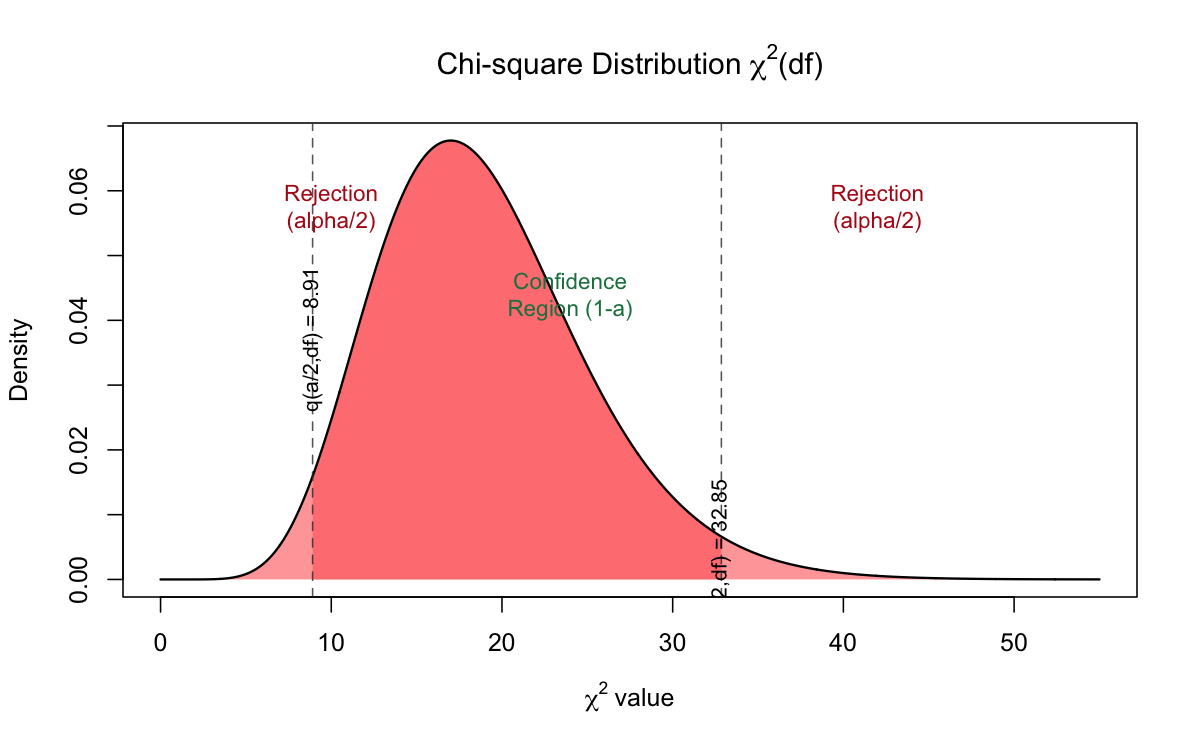
\includegraphics[width=0.75\textwidth]{figures/chi-square-ci.png}
\caption{$\chi^2$ 分布的置信区间示意图。图中阴影区域为置信区间 $[(n-1)S^2/\chi^2_{\alpha/2,n-1}, (n-1)S^2/\chi^2_{1-\alpha/2,n-1}]$ 对应的统计量 $(n-1)S^2/\sigma^2$ 的取值范围，两侧红色区域为显著性水平 $\alpha/2$ 的拒绝域。}
\label{fig:chi-square-ci}
\end{figure}

\section{4.4 Hypothesis Testing}\label{sec:4.4}

假设检验回答一个根本性问题：\textbf{数据是否提供足够证据拒绝关于总体的某个声明？}

这本质上是一种"举证"逻辑：我们先假设某个声明为真（$H_0$），然后问：在这个假设下，当前数据出现的概率有多大？如果概率很小，我们就有理由拒绝这个假设。

\textbf{核心概念}：
\begin{itemize}
\item \textbf{原假设} $H_0$：被检验的假设（通常代表"无效应"或"现状"）
\item \textbf{备择假设} $H_1$：与 $H_0$ 对立的假设
\end{itemize}

在设定假设时，我们需要权衡两类错误：

\begin{center}
\begin{tabular}{c|c|c}
 & 未拒绝 $H_0$ & 拒绝 $H_0$ \\ \hline
$H_0$ 为真 & 正确（置信度 $1-\alpha$） & 第一类错误（概率 $\alpha$） \\
$H_0$ 为假 & 第二类错误（概率 $\beta$） & 正确（功效 $1-\beta$）
\end{tabular}
\end{center}

\textbf{显著性水平}：$\alpha = \mathbb{P}(\text{第一类错误}) = \mathbb{P}(\text{拒绝 } H_0 \mid H_0 \text{ 为真})$

\textbf{自然的问题}：为什么不能同时最小化两类错误？因为在固定样本量下，两类错误是此消彼长的——降低 $\alpha$ 会提高 $\beta$，反之亦然。这正是统计推断中不确定性本质的体现。

\begin{example}[正态均值检验、已知方差]\label{ex:test-normal-known}
设 $X_1, \ldots, X_n \sim N(\mu, \sigma^2)$，$\sigma^2$ 已知。检验 $H_0: \mu = \mu_0$ vs $H_1: \mu > \mu_0$（单侧检验）。

检验统计量：
\[
Z = \frac{\bar{X} - \mu_0}{\sigma/\sqrt{n}}.
\tag{4.4.1}\label{eq:z-test-statistic}\]
\]

在 $\alpha$ 水平下，当 $Z > z_\alpha$ 时拒绝 $H_0$。\footnote{详细推导见附录 \cref{sec:derivation-hypothesis-testing}。}
\end{example}

\begin{example}[正态均值检验、未知方差]\label{ex:test-normal-unknown}
设 $X_1, \ldots, X_n \sim N(\mu, \sigma^2)$，$\sigma^2$ 未知。检验 $H_0: \mu = \mu_0$ vs $H_1: \mu \neq \mu_0$（双侧检验）。

检验统计量：
\[
T = \frac{\bar{X} - \mu_0}{S/\sqrt{n}}.
\tag{4.4.2}\label{eq:t-test-statistic}\]
\]

在 $\alpha$ 水平下，当 $|T| > t_{\alpha/2,n-1}$ 时拒绝 $H_0$。\footnote{详细推导见附录 \cref{sec:derivation-hypothesis-testing}。}
\end{example}

\textbf{$p$ 值}：在 $H_0$ 为真条件下，观察到比当前样本更极端结果的概率。$p$ 值越小，拒绝 $H_0$ 的证据越强。

\textbf{与置信区间的联系}：假设检验和置信区间在本质上是等价的——如果 $\mu_0$ 落在置信区间内，我们就不拒绝 $H_0: \mu = \mu_0$；反之则拒绝。

\section{4.5 Chi-Square Tests}\label{sec:4.5}

直到现在，我们讨论的都是连续型数据。但统计学同样关注\textbf{分类数据（categorical data）}——即计数数据。例如：选举中支持不同候选人的选民人数、不同药物治疗后的治愈/未治愈人数。

\textbf{卡方检验的核心思想}：比较观测频数与期望频数。如果两者差异很大，说明数据可能不服从假设的分布。

\subsection{拟合优度检验}

\textbf{问题}：数据是否来自某个特定分布？

设 $O_1, \ldots, O_k$ 是 $k$ 个类别的观测频数，$E_i = np_{i,0}$ 是 $H_0$ 下的期望频数。

\textbf{检验统计量}：
\[
\chi^2 = \sum_{i=1}^k \frac{(O_i - E_i)^2}{E_i}.
\tag{4.5.1}\label{eq:chi-square-goodness}\]
\]

在 $H_0$ 下，$\chi^2 \approx \chi^2(k-1)$（大样本近似）。拒绝 $H_0$ 当 $\chi^2 > \chi^2_{\alpha, k-1}$。

\textbf{直观理解}：$(O_i - E_i)^2/E_i$ 衡量每个类别的偏差，平方消去正负号，除以 $E_i$ 进行标准化，求和得到总体偏差。\footnote{详细推导见附录 \cref{sec:derivation-chi-square}。}

\begin{figure}[H]
\centering
includegraphics[width=0.7\textwidth]{R/chi-square-goodness.png}
\caption{自由度为 5 的卡方分布，显著性水平 $\alpha=0.05$ 的拒绝域（右侧尾部）。当检验统计量 $\chi^2 > 11.07$ 时，拒绝原假设。}
\label{fig:chi-square-goodness}
\end{figure}

\textbf{例 1：骰子公平性检验}

投掷一枚均匀骰子 $n=600$ 次，观测到各面的次数记录如下：

\begin{center}
\begin{tabular}{c|cccccc|c}
\hline
点数 $i$ & 1 & 2 & 3 & 4 & 5 & 6 & 合计 \\ \hline
观测频数 $O_i$ & 100 & 110 & 95 & 105 & 90 & 100 & 600 \\
\hline
\end{tabular}
\end{center}

如果骰子是均匀的（$H_0$：骰子公平），每个面的期望频数为 $E_i = 600/6 = 100$。

计算 $\chi^2$ 统计量：
\[
\chi^2 = \sum_{i=1}^6 \frac{(O_i - E_i)^2}{E_i}
= \frac{(100-100)^2}{100} + \frac{(110-100)^2}{100} + \frac{(95-100)^2}{100}
+ \frac{(105-100)^2}{100} + \frac{(90-100)^2}{100} + \frac{(100-100)^2}{100}
\]
\[
= 0 + 1 + 0.25 + 0.25 + 1 + 0 = 2.5.
\]

自由度为 $k-1 = 6-1 = 5$。在 $\alpha = 0.05$ 水平，
\[
\chi^2_{0.05, 5} = 11.07.
\]

由于 $\chi^2 = 2.5 < 11.07$，我们\textbf{不拒绝} $H_0$ ——没有足够证据认为这枚骰子不公平。

\textbf{例 2：遗传学中的 Hardy-Weinberg 平衡}

Hardy-Weinberg 平衡（遗传平衡定律）是群体遗传学的基石：在一个随机交配、无选择、无突变、无迁移的群体中，基因型频率将保持世代不变。

设一个二等位基因位点，等位基因频率为 $p$（A）和 $q$（a），则 Hardy-Weinberg 平衡下的基因型期望频率为：
\[
p^2\ (\text{AA}), \quad 2pq\ (\text{Aa}), \quad q^2\ (\text{aa}), \quad p+q=1.
\]

\noindent\textbf{数据}：在某人群中随机调查 300 人，观测到：
\begin{center}
\begin{tabular}{c|ccc|c}
\hline
基因型 & AA & Aa & aa & 合计 \\ \hline
观测频数 $O_i$ & 100 & 50 & 150 & 300 \\
\hline
\end{tabular}
\end{center}

首先由数据估计等位基因频率：
\[
\widehat{p} = \frac{2 \times 100 + 50}{2 \times 300} = \frac{250}{600} \approx 0.417, \quad
\widehat{q} = 1 - \widehat{p} \approx 0.583.
\]

在 Hardy-Weinberg 平衡假设下，期望频数为：
\[
E_{\text{AA}} = 300 \times \widehat{p}^2 = 300 \times 0.417^2 \approx 52.1,
\]
\[
E_{\text{Aa}} = 300 \times 2\widehat{p}\widehat{q} = 300 \times 2 \times 0.417 \times 0.583 \approx 145.8,
\]
\[
E_{\text{aa}} = 300 \times \widehat{q}^2 = 300 \times 0.583^2 \approx 102.1.
\]

计算 $\chi^2$ 统计量：
\[
\chi^2 = \frac{(100-52.1)^2}{52.1} + \frac{(50-145.8)^2}{145.8} + \frac{(150-102.1)^2}{102.1}
\approx 44.1 + 63.0 + 22.5 = 129.6.
\]

自由度为 $k-1 = 3-1 = 2$。在 $\alpha = 0.05$ 水平，$\chi^2_{0.05, 2} = 5.99$。

由于 $\chi^2 = 129.6 > 5.99$，我们\textbf{拒绝} $H_0$ ——该人群的基因型分布显著偏离 Hardy-Weinberg 平衡，可能受到自然选择、突变、迁移或其他进化因素的影响。

\subsection{独立性检验}

对于 $r \times c$ 列联表，设 $O_{ij}$ 为单元格 $(i,j)$ 的观测频数。

在独立性假设下，行合计与列合计的乘积除以总数给出期望频数：
\[
E_{ij} = \frac{O_{i\cdot} O_{\cdot j}}{n}.
\tag{4.5.2}\label{eq:expected-frequency}\]
\]

\textbf{检验统计量}：
\[
\chi^2 = \sum_{i=1}^r\sum_{j=1}^c \frac{(O_{ij} - E_{ij})^2}{E_{ij}}.
\tag{4.5.3}\label{eq:chi-square-independence}\]
\]

在 $H_0$ 下，$\chi^2 \approx \chi^2((r-1)(c-1))$。

\textbf{直观理解}：如果行变量与列变量独立，则每个单元格的观测频数 $O_{ij}$ 应该接近其期望 $E_{ij}$。$\chi^2$ 统计量衡量这种偏离程度——偏离越大，行列不独立的可能性越高。

\textbf{例 3：吸烟与肺癌的关联性检验}

下表记录了 400 人的吸烟状态与肺癌诊断结果：

\begin{center}
\begin{tabular}{c|cc|c}
\hline
 & 肺癌 & 无肺癌 & 合计 \\ \hline
吸烟 & 60 & 140 & 200 \\
不吸烟 & 20 & 180 & 200 \\ \hline
合计 & 80 & 320 & 400 \\
\hline
\end{tabular}
\end{center}

\textbf{研究问题}：吸烟与肺癌是否独立？

在独立性假设下，每个单元格的期望频数为 $E_{ij} = (\text{行合计} \times \text{列合计})/n$：
\[
E_{11} = \frac{200 \times 80}{400} = 40, \quad
E_{12} = \frac{200 \times 320}{400} = 160,
\]
\[
E_{21} = \frac{200 \times 80}{400} = 40, \quad
E_{22} = \frac{200 \times 320}{400} = 160.
\]

计算 $\chi^2$ 统计量：
\[
\chi^2 = \frac{(60-40)^2}{40} + \frac{(140-160)^2}{160}
+ \frac{(20-40)^2}{40} + \frac{(180-160)^2}{160}
\]
\[
= \frac{400}{40} + \frac{400}{160} + \frac{400}{40} + \frac{400}{160}
= 10 + 2.5 + 10 + 2.5 = 25.
\]

自由度为 $(r-1)(c-1) = (2-1)(2-1) = 1$。在 $\alpha = 0.05$ 水平，$\chi^2_{0.05, 1} = 3.84$。

由于 $\chi^2 = 25 > 3.84$，我们\textbf{拒绝} $H_0$ ——吸烟与肺癌之间存在显著关联。进一步计算效应量：
\[
\phi = \sqrt{\frac{\chi^2}{n}} = \sqrt{\frac{25}{400}} = 0.25,
\]
表明吸烟与肺癌之间存在中等强度的正向关联。

\textbf{例 4：两种药物疗效比较}

某制药公司希望比较药物 A 和药物 B 的疗效，将 120 名患者随机分配到两组：

\begin{center}
\begin{tabular}{c|cc|c}
\hline
 & 治愈 & 未治愈 & 合计 \\ \hline
药物 A & 45 & 15 & 60 \\
药物 B & 30 & 30 & 60 \\ \hline
合计 & 75 & 45 & 120 \\
\hline
\end{tabular}
\end{center}

\textbf{研究问题}：两种药物的治愈率是否有显著差异？

在独立性假设下计算期望频数：
\[
E_{11} = \frac{60 \times 75}{120} = 37.5, \quad
E_{12} = \frac{60 \times 45}{120} = 22.5,
\]
\[
E_{21} = \frac{60 \times 75}{120} = 37.5, \quad
E_{22} = \frac{60 \times 45}{120} = 22.5.
\]

计算 $\chi^2$ 统计量：
\[
\chi^2 = \frac{(45-37.5)^2}{37.5} + \frac{(15-22.5)^2}{22.5}
+ \frac{(30-37.5)^2}{37.5} + \frac{(30-22.5)^2}{22.5}
\]
\[
= \frac{56.25}{37.5} + \frac{56.25}{22.5} + \frac{56.25}{37.5} + \frac{56.25}{22.5}
= 1.5 + 2.5 + 1.5 + 2.5 = 8.
\]

自由度为 $(2-1)(2-1) = 1$。在 $\alpha = 0.05$ 水平，$\chi^2_{0.05, 1} = 3.84$。

由于 $\chi^2 = 8 > 3.84$，我们\textbf{拒绝} $H_0$ ——两种药物的疗效存在显著差异。药物 A 的治愈率为 $75\%$，显著高于药物 B 的 $50\%$。

\section{4.6 Monte Carlo Methods}\label{sec:4.6}

有些概率和期望无法解析计算——积分可能没有闭式解，分布可能过于复杂。这时，Monte Carlo 方法提供了一条出路。

\textbf{核心思想}：用随机模拟来近似计算。如果我们可以从某个分布抽样，就可以通过大量重复实验来估计任何期望。

大数定律保证了模拟的收敛性：
\[
\frac{1}{n}\sum_{i=1}^n g(X_i) \xrightarrow{P} \mathbb{E}[g(X)].
\tag{4.6.1}\label{eq:lln-monte-carlo}\]
\]

这意味着：只要模拟次数足够多，样本均值可以任意接近真实期望。

\textbf{接受-拒绝算法}：当目标分布 $f(x)$ 难以直接抽样时，我们可以利用更容易抽样的提议分布 $g(x)$：

\begin{enumerate}
\item 选择提议分布 $g(x)$，满足 $f(x) \leq Mg(x)$（对某个 $M > 1$）
\item 生成 $Y \sim g$ 和 $U \sim \mathrm{Uniform}(0,1)$ 独立
\item 若 $U \leq f(Y)/(Mg(Y))$，接受 $X = Y$；否则拒绝，返回步骤 2
\end{enumerate}

接受概率为 $1/M$。\footnote{接受-拒绝算法的推导及收敛性证明见附录 \cref{sec:derivation-monte-carlo}。}

\section{4.7 Bootstrap Methods}\label{sec:4.7}

\textbf{核心困境}：估计量的抽样分布是统计推断的基础，但这个分布在大多数情况下难以解析计算。例如，样本中位数 $\widehat{m}$ 的分布无法用初等函数表达。

Bootstrap 的解决思路既简单又巧妙：\textbf{用重抽样近似抽样分布}。

\textbf{Bootstrap 的核心假设}：样本就像总体。如果我们有了一个"好"的样本，为什么不从这个样本中有放回地再次抽样，模拟重复实验的过程？

\textbf{步骤}：
\begin{enumerate}
\item 从原始样本中有放回地抽取 $n$ 个观测，形成一个 bootstrap 样本 $X_1^*, \ldots, X_n^*$
\item 计算 bootstrap 复制 $T^* = g(X_1^*, \ldots, X_n^*)$
\item 重复步骤 1-2 多次（如 $B = 1000$ 次），得到 $T_1^*, \ldots, T_B^*$
\item 用 $T_1^*, \ldots, T_B^*$ 的经验分布近似 $T$ 的抽样分布
\end{enumerate}

\textbf{percentile bootstrap 置信区间}：$\theta$ 的 $100(1-\alpha)\%$ 置信区间为
\[
\left[ T_{(\alpha B)}^*,\quad T_{((1-\alpha)B)}^* \right].
\tag{4.7.1}\label{eq:bootstrap-ci}\]
\]

\textbf{直觉}：如果样本是总体的良好代表，那么从样本有放回抽样就是在模拟"从总体中抽取样本"的过程。$T^*$ 的分布反映了 $T$ 的抽样分布的近似。\footnote{Bootstrap 的理论基础及更多细节见附录 \cref{sec:derivation-bootstrap}。}

Bootstrap 的强大之处在于它的通用性——几乎任何估计量都可以用 Bootstrap 近似其分布，不需要繁复的数学推导。这使它成为现代统计实践中的重要工具。

% === 习题 ===
\section*{Exercises}\label{sec:chapter4-exercises}

\begin{exercise}{\ref{exr:4.1.1} Motor Lifetime Data}\label{exr:4.1.1}
Twenty motors were put on test under a high-temperature setting. The lifetimes in hours of the motors under these conditions are given below. Suppose we assume that the lifetime of a motor under these conditions, $X$, has a $\Gamma(1,\theta)$ distribution.

\begin{enumerate}
\item[(a)] Obtain a histogram of the data and overlay it with a density estimate. Based on this plot, do you think that the $\Gamma(1,\theta)$ model is credible?
\item[(b)] Assuming a $\Gamma(1, \theta)$ model, obtain the maximum likelihood estimate $\widehat{\theta}$ of $\theta$ and locate it on your histogram.
\item[(c)] Obtain the sample median of the data. What parameter is it estimating?
\item[(d)] Based on the mle, what is another estimate of the median of $X$?
\end{enumerate}
\end{exercise}

\begin{exercise}{\ref{exr:4.1.2} Baseball Player Weights}\label{exr:4.1.2}
Here are the weights of 26 professional baseball pitchers. Suppose we assume that the weight of a professional baseball pitcher is normally distributed with mean $\mu$ and variance $\sigma^2$.

\begin{enumerate}
\item[(a)] Obtain a histogram of the data. Based on this plot, is a normal probability model credible?
\item[(b)] Obtain the maximum likelihood estimates of $\mu$, $\sigma^2$, $\sigma$, and $\mu/\sigma$.
\item[(c)] Using the binomial model, obtain the maximum likelihood estimate of the proportion $p$ of professional baseball pitchers who weigh over 215 pounds.
\item[(d)] Determine the mle of $p$ assuming that the weight follows the normal probability model $N(\mu, \sigma^2)$.
\end{enumerate}
\end{exercise}

\begin{exercise}{\ref{exr:4.1.3} Poisson Customer Arrivals}\label{exr:4.1.3}
Suppose the number of customers $X$ that enter a store between 9:00 a.m. and 10:00 a.m. follows a Poisson distribution with parameter $\theta$. Suppose a random sample of the number of customers for 10 days results in values: 9, 7, 9, 15, 10, 13, 11, 7, 2, 12.

\begin{enumerate}
\item[(a)] Determine the maximum likelihood estimate of $\theta$. Show that it is an unbiased estimator.
\item[(b)] Based on these data, obtain the realization of your estimator. Explain its meaning.
\end{enumerate}
\end{exercise}

\begin{exercise}{\ref{exr:4.1.4} Verify Likelihood Equations}\label{exr:4.1.4}
For Example 4.1.3, verify equations (4.1.4)-(4.1.8).
\end{exercise}

\begin{exercise}{\ref{exr:4.1.5} Order Statistics Probability}\label{exr:4.1.5}
Let $X_1, X_2, \ldots, X_n$ be a random sample from a continuous-type distribution.
\begin{enumerate}
\item[(a)] Find $P(X_1 \leq X_2)$, $P(X_1 \leq X_2, X_1 \leq X_3)$, $\ldots$, $P(X_1 \leq X_i, i = 2,3,\ldots,n)$.
\item[(b)] Suppose the sampling continues until $X_1$ is no longer the smallest observation. Let $Y$ equal the number of trials (not including $X_1$) until $X_1$ is no longer the smallest. Show that $P(Y = y) = \frac{1}{y(y+1)}$, $y = 1, 2, 3, \ldots$.
\item[(c)] Compute the mean and variance of $Y$ if they exist.
\end{enumerate}
\end{exercise}

\begin{exercise}{\ref{exr:4.1.6} Variance of PMF Estimator}\label{exr:4.1.6}
Consider the estimator of the pmf in expression (4.1.10). We showed that this estimator is unbiased. Find the variance of the estimator and its mgf.
\end{exercise}

\begin{exercise}{\ref{exr:4.1.7} Scottish Schoolchildren Eye Colors}\label{exr:4.1.7}
The data set on Scottish schoolchildren included the eye colors of the children. The frequencies of their eye colors are: Blue: 2978, Light: 6697, Medium: 7511, Dark: 5175. Use these frequencies to obtain a bar chart and an estimate of the associated pmf.
\end{exercise}

\begin{exercise}{\ref{exr:4.1.8} MLE of Poisson PMF}\label{exr:4.1.8}
Assuming that the data in Example 4.1.6 were drawn from a Poisson distribution with mean $\lambda$, obtain the mle of $\lambda$ and then use it to obtain the mle of the pmf. Compare the mle of the pmf to the nonparametric estimate.
\end{exercise}

\begin{exercise}{\ref{exr:4.1.9} Nonparametric Density Estimator}\label{exr:4.1.9}
Consider the nonparametric estimator of a pdf.
\begin{enumerate}
\item[(a)] Obtain its mean and determine the bias of the estimator.
\item[(b)] Obtain the variance of the estimator.
\end{enumerate}
\end{exercise}

\begin{exercise}{\ref{exr:4.1.10} Brain Data Analysis}\label{exr:4.1.10}
This data set consists of a sample of brain information recorded on 40 college students. The variables include gender, height, weight, three IQ measurements, and MRI counts.

\begin{enumerate}
\item[(a)] Load the rda file and print the MRI data.
\item[(b)] Obtain a histogram of the data. Comment on the shape.
\item[(c)] Overlay the default density estimator. Comment on the shape.
\item[(d)] Obtain the sample mean and standard deviation and overlay the normal pdf with these estimates. Comment on the fit.
\item[(e)] Determine the proportions of the data within 1 and 2 standard deviations of the sample mean.
\end{enumerate}
\end{exercise}

\begin{exercise}{\ref{exr:4.1.11} Speed of Light Data}\label{exr:4.1.11}
This is a famous data set on the speed of light recorded by the scientist Simon Newcomb.

\begin{enumerate}
\item[(a)] Load the rda file. Discuss the data.
\item[(b)] Obtain a histogram of the data. Comment on the shape.
\item[(c)] Overlay the default density estimator. Comment on the shape.
\item[(d)] Overlay the normal pdf with sample mean and standard deviation. Comment on the fit.
\item[(e)] Determine the proportions of the data within 1 and 2 standard deviations of the sample mean.
\end{enumerate}
\end{exercise}

\begin{exercise}{\ref{exr:4-12} Normal Confidence Intervals}\label{exr:4-12}
Let the observed value of the mean $\overline{X}$ and of the sample variance of a random sample of size 20 from a distribution that is $N(\mu, \sigma^2)$ be 81.2 and 26.5, respectively. Find respectively $90\%$, $95\%$ and $99\%$ confidence intervals for $\mu$.
\end{exercise}

\begin{exercise}{\ref{exr:4-13} Motor Lifetime Confidence Interval}\label{exr:4-13}
Consider the data on the lifetimes of motors given in Exercise 4.1.1. Obtain a large sample $95\%$ confidence interval for the mean lifetime of a motor.
\end{exercise}

\begin{exercise}{\ref{exr:4-14} Gamma Distribution Inference}\label{exr:4-14}
Suppose we assume that $X_1, X_2, \ldots, X_n$ is a random sample from a $\Gamma(1, \theta)$ distribution.
\begin{enumerate}
\item[(a)] Show that the random variable $(2/\theta)\sum_{i=1}^n X_i$ has a $\chi^2$-distribution with $2n$ degrees of freedom.
\item[(b)] Using the random variable in part (a) as a pivot random variable, find a $(1-\alpha)100\%$ confidence interval for $\theta$.
\item[(c)] Obtain the confidence interval for the data of Exercise 4.1.1.
\end{enumerate}
\end{exercise}

\begin{exercise}{\ref{exr:4-15} Baseball Weight Difference}\label{exr:4-15}
In Example 4.2.4, for the baseball data, find the pooled $t$ $95\%$ confidence interval for the mean difference in weights between the pitchers and hitters.
\end{exercise}

\begin{exercise}{\ref{exr:4-16} Left-handed Baseball Players}\label{exr:4-16}
In the baseball data set, it was found that out of 59 baseball players, 15 were left-handed. Construct a $95\%$ approximate confidence interval for $p$, the proportion of left-handed professional baseball players.
\end{exercise}

\begin{exercise}{\ref{exr:4-17} Sample Size for CI Length}\label{exr:4-17}
Let $\overline{X}$ be the mean of a random sample of size $n$ from a distribution that is $N(\mu, 9)$. Find $n$ such that $P(\overline{X} - 1 < \mu < \overline{X} + 1) = 0.90$, approximately.
\end{exercise}

\begin{exercise}{\ref{exr:4-18} CI from Sample Data}\label{exr:4-18}
Let a random sample of size 17 from the normal distribution $N(\mu, \sigma^2)$ yield $\overline{x} = 4.7$ and $s^2 = 5.76$. Determine a 90\% confidence interval for $\mu$.
\end{exercise}

\begin{exercise}{\ref{exr:4-19} Sample Size for Half-length}\label{exr:4-19}
Let $\overline{X}$ denote the mean of a random sample of size $n$ from a distribution that has mean $\mu$ and variance $\sigma^2 = 10$. Find $n$ so that the probability is approximately 0.954 that the random interval $(\overline{X} - 1/2, \overline{X} + 1/2)$ includes $\mu$.
\end{exercise}

\begin{exercise}{\ref{exr:4-20} Normal CI Length Comparison}\label{exr:4-20}
Let $X_1, X_2, \ldots, X_9$ be a random sample of size 9 from a distribution that is $N(\mu, \sigma^2)$.
\begin{enumerate}
\item[(a)] If $\sigma$ is known, find the length of a $95\%$ confidence interval for $\mu$.
\item[(b)] If $\sigma$ is unknown, find the expected value of the length of a $95\%$ confidence interval for $\mu$.
\item[(c)] Compare these two answers.
\end{enumerate}
\end{exercise}

\begin{exercise}{\ref{exr:4-21} Prediction Interval}\label{exr:4-21}
Let $X_1, X_2, \ldots, X_n, X_{n+1}$ be a random sample of size $n+1$, $n > 1$, from a distribution that is $N(\mu, \sigma^2)$. Find the constant $c$ so that the statistic $c(\overline{X} - X_{n+1})/S$ has a $t$-distribution.
\end{exercise}

\begin{exercise}{\ref{exr:4-22} Monte Carlo CI Coverage}\label{exr:4-22}
Let $X_1, \ldots, X_n$ be a random sample from a $N(0,1)$ distribution. Simulate $m$ confidence intervals and calculate the proportion that trap 0.
\begin{enumerate}
\item[(a)] Set $n=10$ and $m=50$. Run the R code and find the proportion of successful confidence intervals.
\item[(b)] Plot the intervals and comment on the variability of the lengths.
\end{enumerate}
\end{exercise}

\begin{exercise}{\ref{exr:4-23} Invariance of CI Coverage}\label{exr:4-23}
In Exercise 4.2.11, show that setting $\mu=0$ and $\sigma=1$ is without loss of generality.
\end{exercise}

\begin{exercise}{\ref{exr:4-24} Empirical Confidence Level}\label{exr:4-24}
Change the code in the R function getcis so that it also returns the vector ind where ind[i] = 1 if the $i$th confidence interval is successful. Show that the empirical confidence level is mean(ind).
\end{exercise}

\begin{exercise}{\ref{exr:4-25} Gamma CI via CLT}\label{exr:4-25}
Let $\overline{X}$ denote the mean of a random sample of size 25 from a gamma-type distribution with $\alpha=4$ and $\beta>0$. Use the Central Limit Theorem to find an approximate 0.954 confidence interval for $\mu$.
\end{exercise}

\begin{exercise}{\ref{exr:4-26} Sample Size for Given Length}\label{exr:4-26}
Let $\overline{x}$ be the observed mean of a random sample of size $n$ from a distribution having mean $\mu$ and known variance $\sigma^2$. Find $n$ so that $\overline{x} - \sigma/4$ to $\overline{x} + \sigma/4$ is an approximate $95\%$ confidence interval for $\mu$.
\end{exercise}

\begin{exercise}{\ref{exr:4-27} Binomial Sample Size}\label{exr:4-27}
Assume a binomial model for a certain random variable. If we desire a $90\%$ confidence interval for $p$ that is at most 0.02 in length, find $n$.
\end{exercise}

\begin{exercise}{\ref{exr:4-28} Poisson Confidence Interval}\label{exr:4-28}
It is known that a random variable $X$ has a Poisson distribution with parameter $\mu$. A sample of 200 observations from this distribution has a mean equal to 3.4. Construct an approximate $90\%$ confidence interval for $\mu$.
\end{exercise}

\begin{exercise}{\ref{exr:4-29} Variance CI via Chi-square}\label{exr:4-29}
Let $X_1, X_2, \ldots, X_n$ be a random sample from $N(\mu, \sigma^2)$, where both parameters are unknown.
\begin{enumerate}
\item[(a)] Show that $P((n-1)S^2/\sigma^2 < b) = 0.975$ and $P(a < (n-1)S^2/\sigma^2 < b) = 0.95$.
\item[(b)] If $n=9$ and $s^2=7.93$, find a $95\%$ confidence interval for $\sigma^2$.
\item[(c)] If $\mu$ is known, how would you modify the procedure?
\end{enumerate}
\end{exercise}

\begin{exercise}{\ref{exr:4-30} Exact Gamma CI}\label{exr:4-30}
Let $X_1, X_2, \ldots, X_n$ be a random sample from a gamma distribution with known parameter $\alpha=3$ and unknown $\beta>0$. Obtain an exact confidence interval by first obtaining the distribution of $2\sum_{1}^n X_i/\beta$.
\end{exercise}

\begin{exercise}{\ref{exr:4-31} Tack Point-Up Probability}\label{exr:4-31}
When 100 tacks were thrown on a table, 60 of them landed point up. Obtain a $95\%$ confidence interval for the probability that a tack of this type lands point up.
\end{exercise}

\begin{exercise}{\ref{exr:4-32} Two-Sample Normal CI}\label{exr:4-32}
Let two independent random samples, each of size 10, from two normal distributions $N(\mu_1, \sigma^2)$ and $N(\mu_2, \sigma^2)$ yield $\overline{x}=4.8$, $s_1^2=8.64$, $\overline{y}=5.6$, $s_2^2=7.88$. Find a $95\%$ confidence interval for $\mu_1 - \mu_2$.
\end{exercise}

\begin{exercise}{\ref{exr:4-33} Binomial Proportion Difference}\label{exr:4-33}
Let two independent random variables $Y_1$ and $Y_2$ with binomial distributions having parameters $n_1=n_2=100$, $p_1$ and $p_2$, be observed to be $y_1=50$ and $y_2=40$. Determine an approximate $90\%$ confidence interval for $p_1 - p_2$.
\end{exercise}

\begin{exercise}{\ref{exr:4-34} Known Variance Difference}\label{exr:4-34}
Discuss the problem of finding a confidence interval for the difference $\mu_1 - \mu_2$ between the two means of two normal distributions if the variances $\sigma_1^2$ and $\sigma_2^2$ are known but not necessarily equal.
\end{exercise}

\begin{exercise}{\ref{exr:4-35} Unknown Unequal Variance}\label{exr:4-35}
Discuss the problem when the variances are unknown and unequal. If the variances are unknown but their ratio $\sigma_1^2/\sigma_2^2$ is a known constant $k$, then a statistic that is a $T$ random variable can again be used. Why?
\end{exercise}

\begin{exercise}{\ref{exr:4-36} Ratio Known Variance CI}\label{exr:4-36}
Let $X_1, \ldots, X_9$ and $Y_1, \ldots, Y_{12}$ represent two independent random samples from $N(\mu_1, \sigma_1^2)$ and $N(\mu_2, \sigma_2^2)$. It is given that $\sigma_1^2=3\sigma_2^2$, but $\sigma_2^2$ is unknown. Define a random variable that has a $t$-distribution for a $95\%$ confidence interval for $\mu_1 - \mu_2$.
\end{exercise}

\begin{exercise}{\ref{exr:4-37} Sample Size for Mean Difference}\label{exr:4-37}
Let $\overline{X}$ and $\overline{Y}$ be the means of two independent random samples, each of size $n$, from $N(\mu_1, \sigma^2)$ and $N(\mu_2, \sigma^2)$, where the common variance is known. Find $n$ such that $P(\overline{X} - \overline{Y} - \sigma/5 < \mu_1 - \mu_2 < \overline{X} - \overline{Y} + \sigma/5) = 0.90$.
\end{exercise}

\begin{exercise}{\ref{exr:4-38} Variance Ratio CI}\label{exr:4-38}
Let $X_1, \ldots, X_n$ and $Y_1, \ldots, Y_m$ be two independent random samples from $N(\mu_1, \sigma_1^2)$ and $N(\mu_2, \sigma_2^2)$. Construct a confidence interval for the ratio $\sigma_1^2/\sigma_2^2$.
\end{exercise}

\begin{exercise}{\ref{exr:4-39} Exact Binomial CI}\label{exr:4-39}
Recall for the baseball data, 15 out of 59 ballplayers are left-handed. Determine an exact $90\%$ confidence interval for $p$.
\end{exercise}

\begin{exercise}{\ref{exr:4-40} Asymptotic CI Verification}\label{exr:4-40}
In Example 4.3.2, verify the result for the asymptotic confidence interval for $\theta$.
\end{exercise}

\begin{exercise}{\ref{exr:4-41} Discrete Exact Tack CI}\label{exr:4-41}
In Exercise 4.2.20, find the discrete exact confidence interval for the proportion.
\end{exercise}

\begin{exercise}{\ref{exr:4-42} Poisson Exact CI}\label{exr:4-42}
Suppose $X_1, X_2, \ldots, X_{10}$ is a random sample from a Poisson distribution with mean $\theta$. Suppose $n\overline{x}=5$. Compute the exact $90\%$ confidence interval for $\theta$.
\end{exercise}

\begin{exercise}{\ref{exr:4-43} t-Interval Derivation}\label{exr:4-43}
Consider the same setup as in Example 4.3.1 except now assume that $\sigma^2$ is unknown. Set up the equations and derive the $t$-interval for $\theta$.
\end{exercise}

\begin{exercise}{\ref{exr:4-44} Beta Integral Identity}\label{exr:4-44}
Using Exercise 3.3.22, show that
\[
\int_0^p \frac{n!}{(k-1)!(n-k)!} z^{k-1} (1-z)^{n-k} dz = \sum_{w=k}^n \binom{n}{w} p^w (1-p)^{n-w}.
\]
\end{exercise}

\begin{exercise}{\ref{exr:4-45} Poisson CDF Identity}\label{exr:4-45}
This exercise obtains a useful identity for the cdf of a Poisson cdf.
\begin{enumerate}
\item[(a)] Show that
\[
\frac{\lambda^n}{\Gamma(n)} \int_1^\infty x^{n-1} e^{-x\lambda} dx = \sum_{j=0}^{n-1} e^{-\lambda} \frac{\lambda^j}{j!}.
\]
\item[(b)] Obtain the identity used in Example 4.3.3.
\end{enumerate}
\end{exercise}

\begin{exercise}{\ref{exr:4-46} Distribution Quantiles}\label{exr:4-46}
Obtain closed-form expressions for the distribution quantiles based on the exponential and Laplace distributions.
\end{exercise}

\begin{exercise}{\ref{exr:4-47} Potential Outlier Probability}\label{exr:4-47}
Suppose the pdf $f(x)$ is symmetric about 0. Show that the probability of a potential outlier from this distribution is $2F(4q_1)$, where $F^{-1}(0.25)=q_1$. Use this for:
\begin{enumerate}
\item[(a)] The normal distribution.
\item[(b)] The logistic distribution.
\item[(c)] The Laplace distribution.
\end{enumerate}
\end{exercise}

\begin{exercise}{\ref{exr:4-48} Data Summary and Outliers}\label{exr:4-48}
Consider the sample of data: 13, 5, 202, 15, 99, 4, 67, 83, 36, 11, 301, 23, 213, 40, 66, 106, 78, 69, 166, 84, 64.
\begin{enumerate}
\item[(a)] Obtain the five-number summary.
\item[(b)] Determine if there are any outliers.
\item[(c)] Boxplot the data. Comment.
\end{enumerate}
\end{exercise}

\begin{exercise}{\ref{exr:4-49} Normal Q-Q Plot}\label{exr:4-49}
Consider the data in Exercise 4.4.3. Obtain the normal $q$-$q$ plot. Does it suggest the underlying distribution is normal? If not, determine a more appropriate distribution.
\end{exercise}

\begin{exercise}{\ref{exr:4-50} Exponential Order Statistic}\label{exr:4-50}
Let $Y_1 < Y_2 < Y_3 < Y_4$ be the order statistics of a random sample of size 4 from the distribution having pdf $f(x)=e^{-x}$, $0<x<\infty$. Find $P(Y_4 \geq 3)$.
\end{exercise}

\begin{exercise}{\ref{exr:4-51} Continuous Distribution Order Stats}\label{exr:4-51}
Let $X_1, X_2, X_3$ be a random sample from a distribution having pdf $f(x)=2x$, $0<x<1$.
\begin{enumerate}
\item[(a)] Compute the probability that the smallest exceeds the median.
\item[(b)] Find the correlation between $Y_2$ and $Y_3$.
\end{enumerate}
\end{exercise}

\begin{exercise}{\ref{exr:4-52} Discrete Order Statistic PMF}\label{exr:4-52}
Let $f(x)=1/6$, $x=1,2,3,4,5,6$, be the pmf of a discrete distribution. Show that the pmf of the smallest observation of a random sample of size 5 is $g_1(y_1) = (7-y_1)^5/6^5 - (6-y_1)^5/6^5$, $y_1=1,2,\ldots,6$.
\end{exercise}

\begin{exercise}{\ref{exr:4-53} Independent Transformations}\label{exr:4-53}
Let $Y_1 < Y_2 < Y_3 < Y_4 < Y_5$ denote the order statistics from exponential distribution. Show that $Z_1=Y_2$ and $Z_2=Y_4-Y_2$ are independent.
\end{exercise}

\begin{exercise}{\ref{exr:4-54} Beta Distribution of Order Statistic}\label{exr:4-54}
Let $Y_1 < Y_2 < \ldots < Y_n$ be the order statistics from uniform(0,1). Show that $Y_k$ has a beta pdf with parameters $\alpha=k$ and $\beta=n-k+1$.
\end{exercise}

\begin{exercise}{\ref{exr:4-55} Weibull Minimum}\label{exr:4-55}
Let $Y_1 < Y_2 < \ldots < Y_n$ be the order statistics from a Weibull distribution. Find the distribution function and pdf of $Y_1$.
\end{exercise}

\begin{exercise}{\ref{exr:4-56} Uniform Range}\label{exr:4-56}
Find the probability that the range of a random sample of size 4 from the uniform distribution is less than $1/2$.
\end{exercise}

\begin{exercise}{\ref{exr:4-57} Ratio of Order Statistics}\label{exr:4-57}
Let $Y_1 < Y_2 < Y_3$ be order statistics from $f(x)=2x$, $0<x<1$. Show that $Z_1=Y_1/Y_2$, $Z_2=Y_2/Y_3$, and $Z_3=Y_3$ are mutually independent.
\end{exercise}

\begin{exercise}{\ref{exr:4-58} Ratio of Observations}\label{exr:4-58}
Suppose a random sample of size 2 is obtained from $f(x)=2(1-x)$, $0<x<1$. Compute the probability that one sample observation is at least twice as large as the other.
\end{exercise}

\begin{exercise}{\ref{exr:4-59} Midrange Distribution}\label{exr:4-59}
Let $Y_1 < Y_2 < Y_3$ denote order statistics from uniform(0,1). Let $Z=(Y_1+Y_3)/2$ be the midrange. Find the pdf of $Z$.
\end{exercise}

\begin{exercise}{\ref{exr:4-60} Normal Order Stats Expectation}\label{exr:4-60}
Let $Y_1 < Y_2$ denote the order statistics of a random sample of size 2 from $N(0,\sigma^2)$.
\begin{enumerate}
\item[(a)] Show $E(Y_1) = -\sigma/\sqrt{\pi}$.
\item[(b)] Find the covariance of $Y_1$ and $Y_2$.
\end{enumerate}
\end{exercise}

\begin{exercise}{\ref{exr:4-61} Independence Characterizes Exponential}\label{exr:4-61}
Let $Y_1 < Y_2$ be order statistics from a continuous distribution with pdf $f(x)>0$ for $x \geq 0$. Show that the independence of $Z_1=Y_1$ and $Z_2=Y_2-Y_1$ characterizes the gamma pdf with $\alpha=1$.
\end{exercise}

\begin{exercise}{\ref{exr:4-62} Conditional Distribution}\label{exr:4-62}
Let $Y_1 < Y_2 < Y_3 < Y_4$ be order statistics from $f(x)=2x$, $0<x<1$.
\begin{enumerate}
\item[(a)] Find the joint pdf of $Y_3$ and $Y_4$.
\item[(b)] Find the conditional pdf of $Y_3$ given $Y_4=y_4$.
\item[(c)] Evaluate $E(Y_3|y_4)$.
\end{enumerate}
\end{exercise}

\begin{exercise}{\ref{exr:4-63} Triangle Probability}\label{exr:4-63}
Two numbers are selected at random from the interval $(0,1)$. Compute the probability that the three resulting line segments can form a triangle.
\end{exercise}

\begin{exercise}{\ref{exr:4-64} Min and Max Joint PDF}\label{exr:4-64}
Let $X$ and $Y$ be independent with $f(x)=2x$ and $g(y)=3y^2$ on $(0,1)$. Let $U=\min(X,Y)$ and $V=\max(X,Y)$. Find the joint pdf of $U$ and $V$.
\end{exercise}

\begin{exercise}{\ref{exr:4-65} Joint PDF of Min and Max}\label{exr:4-65}
Let the joint pdf of $X$ and $Y$ be $f(x,y)=12x(x+y)/7$, $0<x<1$, $0<y<1$. Let $U=\min(X,Y)$ and $V=\max(X,Y)$. Find the joint pdf of $U$ and $V$.
\end{exercise}

\begin{exercise}{\ref{exr:4-66} Gini's Mean Difference}\label{exr:4-66}
Let $X_1, X_2, \ldots, X_n$ be a random sample. Gini's mean difference is $G = \sum_{j=2}^n \sum_{i=1}^{j-1} |X_i-X_j| / \binom{n}{2}$.
\begin{enumerate}
\item[(a)] If $n=10$, find $a_1, \ldots, a_{10}$ so that $G = \sum_{i=1}^{10} a_i Y_i$.
\item[(b)] Show $E(G) = 2\sigma/\sqrt{\pi}$ for normal distribution.
\end{enumerate}
\end{exercise}

\begin{exercise}{\ref{exr:4-67} Exponential Order Stats Properties}\label{exr:4-67}
Let $Y_1 < Y_2 < \ldots < Y_n$ be order statistics from exponential distribution.
\begin{enumerate}
\item[(a)] Show $Z_1=nY_1$, $Z_2=(n-1)(Y_2-Y_1)$, $Z_3=(n-2)(Y_3-Y_2)$, $\ldots$, $Z_n=Y_n-Y_{n-1}$ are independent exponentials.
\item[(b)] Demonstrate that all linear functions of $Y_i$ can be expressed as linear functions of independent random variables.
\end{enumerate}
\end{exercise}

\begin{exercise}{\ref{exr:4-68} PERT Distribution}\label{exr:4-68}
In PERT, let $X_1, X_2, X_3$ be three independent uniform random times. For series completion ($Y=X_1+X_2+X_3$) and parallel completion ($Z=\max(X_1,X_2,X_3)$)), find their pdfs.
\end{exercise}

\begin{exercise}{\ref{exr:4-69} Sample Size for Extreme Quantile}\label{exr:4-69}
Let $Y_n$ denote the $n$th order statistic. Find the smallest $n$ for which $P(\xi_{0.9} < Y_n) \geq 0.75$.
\end{exercise}

\begin{exercise}{\ref{exr:4-70} Probability Involving Quantiles}\label{exr:4-70}
Let $Y_1 < Y_2 < Y_3 < Y_4 < Y_5$ denote order statistics of size 5. Compute:
\begin{enumerate}
\item[(a)] $P(Y_1 < \xi_{0.5} < Y_5)$
\item[(b)] $P(Y_1 < \xi_{0.25} < Y_3)$
\item[(c)] $P(Y_4 < \xi_{0.80} < Y_5)$
\end{enumerate}
\end{exercise}

\begin{exercise}{\ref{exr:4-71} Median Between Order Stats}\label{exr:4-71}
Compute $P(Y_3 < \xi_{0.5} < Y_7)$ if $Y_1 < \ldots < Y_9$ are order statistics of size 9.
\end{exercise}

\begin{exercise}{\ref{exr:4-72} Sample Size for Median Coverage}\label{exr:4-72}
Find the smallest $n$ for which $P(Y_1 < \xi_{0.5} < Y_n) \geq 0.99$.
\end{exercise}

\begin{exercise}{\ref{exr:4-73} Normal Order Stats Interval}\label{exr:4-73}
Let $Y_1 < Y_2$ be order statistics from $N(\mu,\sigma^2)$ with known $\sigma^2$.
\begin{enumerate}
\item[(a)] Show $P(Y_1 < \mu < Y_2) = 1/2$ and compute $E(Y_2-Y_1)$.
\item[(b)] Find $c$ such that $P(\overline{X}-c\sigma < \mu < \overline{X}+c\sigma) = 1/2$.
\end{enumerate}
\end{exercise}

\begin{exercise}{\ref{exr:4-74} Selection Algorithm}\label{exr:4-74}
Let $y_1 < y_2 < y_3$ be observed order statistics. A statistician is given these values in random order and wants to select the largest. She looks at the first but refuses it and then takes the second if larger than the first, else takes the third. Show this algorithm has probability $1/2$ of selecting the largest.
\end{exercise}

\begin{exercise}{\ref{exr:4-75} Motor Median CI}\label{exr:4-75}
Refer to Exercise 4.1.1. Using expression (4.4.10), obtain a confidence interval for the median lifetime of a motor.
\end{exercise}

\begin{exercise}{\ref{exr:4-76} Power Function of Test}\label{exr:4-76}
Show that the approximate power function given in expression (4.5.12) is strictly increasing. Show the test has approximate size $\alpha$ for testing $H_0: \mu \leq \mu_0$ vs $H_1: \mu > \mu_0$.
\end{exercise}

\begin{exercise}{\ref{exr:4-77} Darwin Data t-Test}\label{exr:4-77}
For the Darwin data, verify that the Student $t$-test statistic is 2.15.
\end{exercise}

\begin{exercise}{\ref{exr:4-78} Neyman-Pearson Test}\label{exr:4-78}
Let $X$ have pdf $f(x;\theta) = \theta x^{\theta-1}$, $0<x<1$. To test $H_0: \theta=1$ against $H_1: \theta=2$, use critical region $C=\{(x_1,x_2): x_1x_2 \geq 3/4\}$. Find the power function.
\end{exercise}

\begin{exercise}{\ref{exr:4-79} Binomial Significance Level}\label{exr:4-79}
Let $X$ have binomial distribution with $n=10$ and $p=1/4$ or $1/2$. Test $H_0: p=1/2$ vs $H_1: p=1/4$ by rejecting if $X_1 \leq 3$. Find significance level and power.
\end{exercise}

\begin{exercise}{\ref{exr:4-80} Exponential LR Test}\label{exr:4-80}
Let $X_1,X_2$ be a sample from $f(x;\theta)=(1/\theta)e^{-x/\theta}$. Reject $H_0: \theta=2$ if $f(x_1;2)f(x_2;2)/[f(x_1;1)f(x_2;1)] \leq 1/2$. Find significance level and power when $H_0$ is false.
\end{exercise}

\begin{exercise}{\ref{exr:4-81} Power Curve Sketch}\label{exr:4-81}
Consider tests Test 1 and Test 2. For Test A, reject $H_0$ if $S \leq k_A$; for Test B, reject if $S \leq k_B$. If Test A has higher significance level, show Test A has higher power.
\end{exercise}

\begin{exercise}{\ref{exr:4-82} Tire Life Test}\label{exr:4-82}
Let tire life $X \sim N(\theta, 5000^2)$. Test $H_0: \theta=30000$ vs $H_1: \theta>30000$. Determine $n$ and $c$ so that $\gamma(30000)=0.01$ and $\gamma(35000)=0.98$.
\end{exercise}

\begin{exercise}{\ref{exr:4-83} Poisson Power Function}\label{exr:4-83}
Let $X$ have Poisson distribution. Test $H_0: \theta=1/2$ vs $H_1: \theta<1/2$. With $n=12$, reject if $Y=\sum X_i \leq 2$. Graph the power function and determine significance level.
\end{exercise}

\begin{exercise}{\ref{exr:4-84} Binomial Sample Size}\label{exr:4-84}
Let $Y \sim \text{binomial}(n,p)$. Test $H_0: p=1/2$ vs $H_1: p>1/2$. Find $n$ and $c$ so that $\gamma(1/2)=0.10$ and $\gamma(2/3)=0.95$.
\end{exercise}

\begin{exercise}{\ref{exr:4-85} Uniform Max Test}\label{exr:4-85}
Let $Y_1<Y_2<Y_3<Y_4$ be order statistics from $f(x;\theta)=1/\theta$, $0<x<\theta$. Test $H_0: \theta=1$ vs $H_1: \theta>1$ by rejecting if $Y_4 \geq c$.
\begin{enumerate}
\item[(a)] Find $c$ for $\alpha=0.05$.
\item[(b)] Determine the power function.
\end{enumerate}
\end{exercise}

\begin{exercise}{\ref{exr:4-86} Poisson Test Size}\label{exr:4-86}
Let $X_1,\ldots,X_8$ be from Poisson with mean $\mu$. Test $H_0: \mu=0.5$ vs $H_1: \mu>0.5$ by rejecting if $\sum x_i \geq 8$.
\begin{enumerate}
\item[(a)] Show significance level is $1-\text{ppois}(7,4)$.
\item[(b)] Determine $\gamma(0.75)$, $\gamma(1)$, $\gamma(1.25)$.
\end{enumerate}
\end{exercise}

\begin{exercise}{\ref{exr:4-87} Tennis Serve Hypothesis}\label{exr:4-87}
Let $p$ be probability that first serve is good. Test $H_0: p=0.40$ vs $H_1: p>0.40$ with $n=25$. Reject if $Y \geq 13$.
\begin{enumerate}
\item[(a)] Show $\alpha = 1-\text{pbinom}(12,25,0.4)$.
\item[(b)] Find $\beta$ when $p=0.60$.
\end{enumerate}
\end{exercise}

\begin{exercise}{\ref{exr:4-88} Bernoulli Power Comparison}\label{exr:4-88}
Let $S$ be number of successes in $n=40$ Bernoulli trials. Test $H_0: p \leq 0.3$ vs $H_1: p > 0.3$. Compare tests: (1) Reject if $S \geq 16$ and (2) Reject if $S \geq 17$. Determine levels.
\end{exercise}

\begin{exercise}{\ref{exr:4-89} Proportion Power Curve}\label{exr:4-89}
Consider the two-sided test for proportions. Write R code to compute a plot of the power curve.
\end{exercise}

\begin{exercise}{\ref{exr:4-90} Power Function Derivative}\label{exr:4-90}
Consider the power function $\gamma(\mu)$. Show $\gamma'(\mu)$ is strictly negative for $\mu < \mu_0$ and strictly positive for $\mu > \mu_0$.
\end{exercise}

\begin{exercise}{\ref{exr:4-91} Exact Size t-Test}\label{exr:4-91}
Show that the test defined by (4.6.9) has exact size $\alpha$ for testing $H_0: \mu = \mu_0$ vs $H_1: \mu \neq \mu_0$.
\end{exercise}

\begin{exercise}{\ref{exr:4-92} One vs Two-Sided Power}\label{exr:4-92}
Consider the one-sided $t$-test and two-sided $t$-test, both of size $\alpha$. Show that for $\mu > \mu_0$, the power function of the one-sided test is larger.
\end{exercise}

\begin{exercise}{\ref{exr:4-93} Paired Design Analysis}\label{exr:4-93}
A baseball coach paired 20 members by speed. Data on self vs rival times are given.
\begin{enumerate}
\item[(a)] Obtain comparison boxplots. Comment.
\item[(b)] Compute paired $t$-test and $p$-value.
\item[(c)] Obtain point estimate and $95\%$ CI for $\mu_d$.
\item[(d)] Conclude.
\end{enumerate}
\end{exercise}

\begin{exercise}{\ref{exr:4-94} AZT Dosage Study}\label{exr:4-94}
A data set concerning the effect of AZT dosages on HIV patients. Compare $300$mg and $600$mg groups.
\begin{enumerate}
\item[(a)] Obtain comparison boxplots.
\item[(b)] Compute two-sample $t$-test and $p$-value.
\item[(c)] Obtain point estimate and $95\%$ CI for $\Delta$.
\item[(d)] Conclude.
\end{enumerate}
\end{exercise}

\begin{exercise}{\ref{exr:4-95} Air Quality Comparison}\label{exr:4-95}
Compare suspended particle concentrations between Melbourne and Houston. Test $H_0: \mu_X = \mu_Y$ against $H_1: \mu_X < \mu_Y$.
\begin{enumerate}
\item[(a)] Define test statistic and critical region.
\item[(b)] Calculate with given statistics.
\end{enumerate}
\end{exercise}

\begin{exercise}{\ref{exr:4-96} Seat Belt Campaign}\label{exr:4-96}
Let $p$ be proportion of drivers using seat belts. After campaign, $y=104$ out of $n=590$ wore belts. Was campaign successful?
\begin{enumerate}
\item[(a)] Define hypotheses.
\item[(b)] Critical region at $\alpha=0.01$.
\item[(c)] Determine $p$-value.
\end{enumerate}
\end{exercise}

\begin{exercise}{\ref{exr:4-97} Variance Test Critical Value}\label{exr:4-97}
Test $H_0: \sigma^2 = \sigma_0^2$ against $H_1: \sigma^2 > \sigma_0^2$ using critical region $(n-1)S^2/\sigma_0^2 \geq c$. If $n=13$ and $\alpha=0.025$, determine $c$.
\end{exercise}

\begin{exercise}{\ref{exr:4-98} F-Test Critical Value}\label{exr:4-98}
Test $H_0: \sigma_1^2 = \sigma_2^2$ against $H_1: \sigma_1^2 > \sigma_2^2$ using $F \geq c$. If $n=13$, $m=11$, and $\alpha=0.05$, find $c$.
\end{exercise}

\begin{exercise}{\ref{exr:4-99} Modified Frequency Test}\label{exr:4-99}
Suppose observed frequencies of $A_1,\ldots,A_4$ are 20, 30, 92, 105. Calculate the test and report $p$-value.
\end{exercise}

\begin{exercise}{\ref{exr:4-100} Continuous Interval Test}\label{exr:4-100}
A number is selected from $(0,2)$. Test hypothesis with $p_{i0} = \int_{A_i} (1/2)(2-x)dx$. For observed frequencies 30, 30, 10, 10, would $H_0$ be accepted?
\end{exercise}

\begin{exercise}{\ref{exr:4-101} Normal Approximation Test}\label{exr:4-101}
Define sets $A_1=\{x:-\infty<x\leq 0\}$, $A_i=\{x:i-2<x\leq i-1\}$ for $i=2,\ldots,7$, $A_8=\{x:6<x<\infty\}$. Test with frequencies 60, 96, 140, 210, 172, 160, 88, 74.
\end{exercise}

\begin{exercise}{\ref{exr:4-102} Die Casting Test}\label{exr:4-102}
A die was cast $n=120$ times with frequencies: 1:$b$, 2:20, 3:20, 4:20, 5:20, 6:$40-b$. For what values of $b$ would the hypothesis of unbiased die be rejected at $0.025$ level?
\end{exercise}

\begin{exercise}{\ref{exr:4-103} Mendelian Genetics}\label{exr:4-103}
Mendelian theory states probabilities are 9/16, 3/16, 3/16, 1/16 for four classifications. With observed frequencies 86, 35, 26, 13 out of 160, test at $\alpha=0.01$.
\end{exercise}

\begin{exercise}{\ref{exr:4-104} Teaching Method Comparison}\label{exr:4-104}
Two groups of 100 students each. Test at $5\%$ whether the two distributions are the same.
\end{exercise}

\begin{exercise}{\ref{exr:4-105} Crime and Alcoholism}\label{exr:4-105}
Data on crime type and alcoholic status. Test independence.
\begin{enumerate}
\item[(a)] Compute $\chi^2$-test for independence.
\item[(b)] Use Pearson residuals to determine strongest dependence.
\item[(c)] Confirm with conditional test.
\end{enumerate}
\end{exercise}

\begin{exercise}{\ref{exr:4-106} Independence Test}\label{exr:4-106}
180 independent trials with classification into $A_1,A_2,A_3$ and $B_1,B_2,B_3,B_4$. What is smallest $k$ that leads to rejection at $\alpha=0.05$?
\end{exercise}

\begin{exercise}{\ref{exr:4-107} Poisson Goodness of Fit}\label{exr:4-107}
Fit Poisson distribution to data: x: 0,1,2,3,3<x with frequencies 20,40,16,18,6.
\begin{enumerate}
\item[(a)] Compute chi-square statistic.
\item[(b)] Degrees of freedom?
\item[(c)] Reject at $\alpha=0.05$?
\end{enumerate}
\end{exercise}

\begin{exercise}{\ref{exr:4-108} MCT Converse}\label{exr:4-108}
Prove the converse of Theorem MCT: Let $X$ have continuous cdf $F(x)$ strictly increasing. Show $Z=F(X)$ has uniform(0,1) distribution.
\end{exercise}

\begin{exercise}{\ref{exr:4-109} Monte Carlo Log 2}\label{exr:4-109}
Approximate $\log 2 = \int_0^1 1/(x+1) dx$ using uniform(0,1) generator. Write R function and compare with true value.
\end{exercise}

\begin{exercise}{\ref{exr:4-110} Normal CDF Approximation}\label{exr:4-110}
Approximate $\int_0^{1.96} (1/\sqrt{2\pi}) \exp\{-t^2/2\} dt$ using Monte Carlo.
\end{exercise}

\begin{exercise}{\ref{exr:4-111} Location-Scale Generation}\label{exr:4-111}
Suppose $X$ has pdf $f_X(x) = b^{-1} f((x-a)/b)$. If we can generate from $f(z)$, explain how to generate from $f_X(x)$.
\end{exercise}

\begin{exercise}{\ref{exr:4-112} Logistic Distribution Generation}\label{exr:4-112}
Determine a method to generate random observations for the logistic pdf. Write R function and verify with histogram.
\end{exercise}

\begin{exercise}{\ref{exr:4-113} Beta Generator}\label{exr:4-113}
Determine a method to generate random observations for $f(x)=4x^3$, $0<x<1$. Write R function.
\end{exercise}

\begin{exercise}{\ref{exr:4-114} Laplace Inverse CDF}\label{exr:4-114}
Obtain the inverse function of the cdf of the Laplace pdf $f(x)=(1/2)e^{-|x|}$. Write R function.
\end{exercise}

\begin{exercise}{\ref{exr:4-115} Extreme Value Generation}\label{exr:4-115}
Determine a method to generate random observations for the extreme-valued pdf $f(x)=\exp\{x-e^x\}$. Write R function.
\end{exercise}

\begin{exercise}{\ref{exr:4-116} Cauchy Distribution}\label{exr:4-116}
Determine a method to generate random observations for the Cauchy distribution $f(x)=1/[\pi(1+x^2)]$. Write R function.
\end{exercise}

\begin{exercise}{\ref{exr:4-117} Weibull Generation}\label{exr:4-117}
Determine a method to generate random observations for the Weibull distribution. Write R function.
\end{exercise}

\begin{exercise}{\ref{exr:4-118} Contaminated Normal Power}\label{exr:4-118}
Write algorithm to simulate power of the test for contaminated normal distribution. Modify R function.
\end{exercise}

\begin{exercise}{\ref{exr:4-119} Logistic Power Simulation}\label{exr:4-119}
Write algorithm to simulate significance level and power for logistic distribution.
\end{exercise}

\begin{exercise}{\ref{exr:4-120} General Inverse CDF}\label{exr:4-120}
For cdf $F(x)$ not strictly increasing, define $F^{-1}(u)=\inf\{x: F(x) \geq u\}$. Let $U \sim \text{uniform}(0,1)$. Prove $F^{-1}(U)$ has cdf $F(x)$.
\end{exercise}

\begin{exercise}{\ref{exr:4-121} Ratio Maximum}\label{exr:4-121}
Verify the derivative in (4.8.12) and show the function attains maximum at $x=(\alpha-[\alpha])/(1-b)$.
\end{exercise}

\begin{exercise}{\ref{exr:4-122} Minimum Derivation}\label{exr:4-122}
Derive expression (4.8.14) and show $b=[\alpha]/\alpha$ gives minimum.
\end{exercise}

\begin{exercise}{\ref{exr:4-123} Gamma via Beta}\label{exr:4-123}
Assume $Y_1 \sim \Gamma(\alpha+1,1)$, $Y_2 \sim \text{uniform}(0,1)$. Let $X_1=Y_1 Y_2^{1/\alpha}$ and $X_2=Y_2$. Show $X_1 \sim \Gamma(\alpha,1)$.
\end{exercise}

\begin{exercise}{\ref{exr:4-124} Ratio Derivative}\label{exr:4-124}
Show the derivative of the ratio in (4.8.10) is $-x\exp\{-x^2/2\}(x^2-1)$ with critical values $\pm 1$.
\end{exercise}

\begin{exercise}{\ref{exr:4-125} Beta Distribution Generation}\label{exr:4-125}
Consider accept-reject algorithm for beta distribution. Show $X$ has beta distribution with parameters $\alpha$ and $\beta$.
\end{exercise}

\begin{exercise}{\ref{exr:4-126} Marsaglia-Bray Normal}\label{exr:4-126}
Consider the Marsaglia-Bray algorithm for generating normal random variables. Show $X_1$ and $X_2$ are iid $N(0,1)$.
\end{exercise}

\begin{exercise}{\ref{exr:4-127} Bootstrap CI for Mean}\label{exr:4-127}
Use the R function percentcboot to obtain a bootstrap $95\%$ confidence interval for the mean concentration. Compare with $t$-CI.
\end{exercise}

\begin{exercise}{\ref{exr:4-128} Bootstrap Sample Properties}\label{exr:4-128}
Let $x_1^*, \ldots, x_n^*$ be a bootstrap sample drawn with replacement.
\begin{enumerate}
\item[(a)] Show $x_i^*$ are iid with common cdf $\widehat{F}_n$.
\item[(b)] Show $E(x_i^*) = \overline{x}$.
\item[(c)] If $n$ odd, show $\text{median}\{x_i^*\} = x_{(n+1)/2}$.
\item[(d)] Show $V(x_i^*) = n^{-1}\sum(x_i-\overline{x})^2$.
\end{enumerate}
\end{exercise}

\begin{exercise}{\ref{exr:4-129} Gamma Bootstrap CI}\label{exr:4-129}
Let $X_1,\ldots,X_n \sim \Gamma(1,\beta)$.
\begin{enumerate}
\item[(a)] Show $(2n\overline{X}/(\chi_{2n}^2)^{(1-\alpha/2)}, 2n\overline{X}/(\chi_{2n}^2)^{(\alpha/2)})$ is exact CI for $\beta$.
\item[(b)] Show $90\%$ CI for data is (64.99, 136.69).
\end{enumerate}
\end{exercise}

\begin{exercise}{\ref{exr:4-130} Bootstrap Median CI}\label{exr:4-130}
Suppose we want to estimate the median using sample median. Obtain $90\%$ bootstrap percentile CI. Did it trap the true median?
\end{exercise}

\begin{exercise}{\ref{exr:4-131} Bootstrap t-Interval}\label{exr:4-131}
Suppose $X_1,\ldots,X_n \sim N(\mu,\sigma^2)$. Show the pivot $t = (\overline{X}-\mu)/(S/\sqrt{n})$ leads to CI.
\end{exercise}

\begin{exercise}{\ref{exr:4-132} Standardized Bootstrap CI}\label{exr:4-132}
Consider bootstrap pivot $t^* = (\overline{x}^* - \overline{x})/(s^*/\sqrt{n})$.
\begin{enumerate}
\item[(a)] Rewrite percentile CI algorithm using $t^*$.
\item[(b)] Find $90\%$ CI for data in Example 4.9.3.
\item[(c)] Compare with nonstandardized CI.
\end{enumerate}
\end{exercise}

\begin{exercise}{\ref{exr:4-133} Bootstrap Median Test}\label{exr:4-133}
Consider algorithm for two-sample bootstrap test based on difference in medians.
\begin{enumerate}
\item[(a)] Rewrite algorithm for median.
\item[(b)] Obtain bootstrap test.
\item[(c)] Compare $p$-value with 0.063.
\end{enumerate}
\end{exercise}

\begin{exercise}{\ref{exr:4-134} Two-Sample t-Test Value}\label{exr:4-134}
Consider data of Example 4.9.2. Show $t=0.93$ with $p$-value 0.18.
\end{exercise}

\begin{exercise}{\ref{exr:4-135} Bootstrap Two-Sided Test}\label{exr:4-135}
In Example 4.9.3, test $H_0: \mu=90$ vs $H_1: \mu \neq 90$.
\begin{enumerate}
\item[(a)] Determine bootstrap $p$-value.
\item[(b)] Rewrite R program.
\item[(c)] Compute $p$-value with 3000 bootstraps.
\end{enumerate}
\end{exercise}

\begin{exercise}{\ref{exr:4-136} Permutation Test}\label{exr:4-136}
Consider permutation test for two-sample problem.
\begin{enumerate}
\item[(a)] For $x'=(10,15,21)$ and $y'=(20,25,30)$, determine $p$-value.
\item[(b)] Approximate permutation test with 3000 resamples.
\item[(c)] Probability of distinct samples?
\end{enumerate}
\end{exercise}

\begin{exercise}{\ref{exr:4-137} Bootstrap z Distribution}\label{exr:4-137}
Let $z^*$ be drawn from discrete distribution with mass $n^{-1}$ at $z_i = x_i - \overline{x} + \mu_0$. Determine $E(z^*)$ and $V(z^*)$.
\end{exercise}

\begin{exercise}{\ref{exr:4-138} Bootstrap t-Test Value}\label{exr:4-138}
For Example 4.9.3, show $t=0.84$ and $p$-value is 0.20.
\end{exercise}

\begin{exercise}{\ref{exr:4-139} Bootstrap Median Test}\label{exr:4-139}
For Example 4.9.3, obtain bootstrap test based on medians for $H_0: \mu=90$ vs $H_1: \mu>90$.
\end{exercise}

\begin{exercise}{\ref{exr:4-140} Darwin Experiment Bootstrap}\label{exr:4-140}
Consider Darwin's experiment on Zea mays.
\begin{enumerate}
\item[(a)] Obtain bootstrap test keeping pairing intact.
\item[(b)] Write R program and compare $p$-value.
\end{enumerate}
\end{exercise}

\section*{本章小结}

\textbf{核心概念}：
\begin{itemize}
\item \textbf{统计量}：样本的函数，不依赖未知参数
\item \textbf{点估计}：MLE、矩估计；无偏性、偏差
\item \textbf{置信区间}：参数的合理取值范围；宽度随样本量增大而减小
\item \textbf{假设检验}：第一类和第二类错误的权衡
\end{itemize}

\textbf{重要公式}：
\begin{center}
\begin{tabular}{|c|c|}
\hline
\textbf{场景} & \textbf{置信区间/检验统计量} \\ \hline
正态均值、已知 $\sigma$ & $\bar{X} \pm z_{\alpha/2}\sigma/\sqrt{n}$ \\ \hline
正态均值、未知 $\sigma$ & $\bar{X} \pm t_{\alpha/2,n-1}S/\sqrt{n}$ \\ \hline
正态方差 & $\frac{(n-1)S^2}{\chi^2_{\alpha/2,n-1}},\frac{(n-1)S^2}{\chi^2_{1-\alpha/2,n-1}}$ \\ \hline
单样本 $Z$ 检验 & $Z = \frac{\bar{X}-\mu_0}{\sigma/\sqrt{n}}$ \\ \hline
单样本 $t$ 检验 & $T = \frac{\bar{X}-\mu_0}{S/\sqrt{n}}$ \\ \hline
拟合优度 $\chi^2$ & $\chi^2 = \sum \frac{(O-E)^2}{E} \approx \chi^2(k-1)$ \\ \hline
\end{tabular}
\end{center}

\section{附录：公式推导}\label{sec:appendix-derivation}

\subsection{通用 MLE 推导}\label{sec:derivation-mle}

\textbf{背景}：最大似然估计的通用推导框架。

\textbf{核心思想}：MLE 选择使似然函数最大化的参数值。在正则条件下，MLE 满足似然方程 $\frac{\partial l(\theta)}{\partial \theta} = 0$。

\textbf{渐近性质}（不证）：
在温和条件下，$\widehat{\theta}$ 具有以下渐近性质：
\begin{enumerate}
\item \textbf{一致性}：$\widehat{\theta} \xrightarrow{P} \theta$
\item \textbf{渐近正态性}：$\sqrt{n}(\widehat{\theta} - \theta) \Rightarrow \mathcal{N}(0, I(\theta)^{-1})$，其中 $I(\theta)$ 是 Fisher 信息量
\item \textbf{渐近有效性}：方差达到 Cram\'er-Rao 下界
\end{enumerate}

这些性质使 MLE 成为现代统计推断的基石。

\subsection{指数分布 MLE 的推导}\label{sec:derivation-exponential-mle}

\textbf{背景}：设 $X_1, \ldots, X_n \sim \mathrm{Exp}(\theta)$，即 $f(x) = \theta^{-1}\exp\{-x/\theta\}$，$x > 0$。

\textbf{目标}：求使似然函数最大化的 $\theta$ 值。

\textbf{推导步骤}：

1. 似然函数为
\[
L(\theta) = \prod_{i=1}^{n} \theta^{-1}\exp\{-x_i/\theta\} = \theta^{-n}\exp\{-\theta^{-1}\sum_{i=1}^{n}x_i\}.
\]

2. 对数似然函数为
\[
l(\theta) = -n\log\theta - \theta^{-1}\sum_{i=1}^{n}x_i.
\]

3. 求导并设为零：
\[
\frac{\partial l(\theta)}{\partial \theta} = -\frac{n}{\theta} + \frac{1}{\theta^2}\sum_{i=1}^{n}x_i = 0.
\]

4. 解得
\[
\widehat{\theta} = \frac{1}{n}\sum_{i=1}^{n}x_i = \bar{x}.
\]

5. 验证这是最大值（二阶导数为负）：
\[
\frac{\partial^2 l(\theta)}{\partial \theta^2} = \frac{n}{\theta^2} - \frac{2}{\theta^3}\sum_{i=1}^{n}x_i = -\frac{n}{\theta^2} < 0.
\]

\textbf{结论}：$\widehat{\theta} = \bar{X}$ 是 $\theta$ 的 MLE。由于 $\mathbb{E}(X) = \theta$，故它也是无偏的。

\subsection{二项分布 MLE 的推导}\label{sec:derivation-binomial-mle}

\textbf{背景}：设 $X \sim \mathrm{Bernoulli}(\theta)$，对于随机样本 $X_1, \ldots, X_n$。

\textbf{目标}：求 $\theta$ 的 MLE。

\textbf{推导步骤}：

1. 似然函数为
\[
L(\theta) = \prod_{i=1}^{n} \theta^{x_i}(1-\theta)^{1-x_i} = \theta^{\sum x_i}(1-\theta)^{n-\sum x_i}.
\]

2. 对数似然函数为
\[
l(\theta) = \left(\sum_{i=1}^{n} x_i\right)\log\theta + \left(n - \sum_{i=1}^{n} x_i\right)\log(1-\theta).
\]

3. 求导并设为零：
\[
\frac{\partial l(\theta)}{\partial \theta} = \frac{\sum x_i}{\theta} - \frac{n - \sum x_i}{1-\theta} = 0.
\]

4. 解得
\[
\widehat{\theta} = \frac{1}{n}\sum_{i=1}^{n} x_i = \bar{x}.
\]

\textbf{结论}：样本均值（样本比例）是 $\theta$ 的 MLE，也是无偏估计。

\subsection{正态分布 MLE 的推导}\label{sec:derivation-normal-mle}

\textbf{背景}：设 $X \sim \mathcal{N}(\mu, \sigma^2)$，对于随机样本。

\textbf{目标}：求 $\mu$ 和 $\sigma^2$ 的 MLE。

\textbf{推导步骤}：

1. 对数似然函数为
\[
l(\mu, \sigma) = -\frac{n}{2}\log 2\pi - n\log\sigma - \frac{1}{2}\sum_{i=1}^{n}\left(\frac{x_i-\mu}{\sigma}\right)^2.
\]

2. 对 $\mu$ 求偏导并设为零：
\[
\frac{\partial l}{\partial \mu} = -\frac{1}{\sigma^2}\sum_{i=1}^{n}(x_i - \mu) = 0 \implies \widehat{\mu} = \bar{x}.
\]

3. 对 $\sigma$ 求偏导并设为零（先代入 $\widehat{\mu}$）：
\[
\frac{\partial l}{\partial \sigma} = -\frac{n}{\sigma} + \frac{1}{\sigma^3}\sum_{i=1}^{n}(x_i - \bar{x})^2 = 0 \implies \widehat{\sigma}^2 = \frac{1}{n}\sum_{i=1}^{n}(x_i - \bar{x})^2.
\]

\textbf{注意}：$\widehat{\sigma}^2$ 是有偏的，因为
\[
\mathbb{E}[\widehat{\sigma}^2] = \frac{n-1}{n}\sigma^2.
\]
无偏估计为 $S^2 = \frac{n}{n-1}\widehat{\sigma}^2$。

\subsection{置信区间推导汇总}\label{sec:derivation-confidence-interval}

\textbf{背景}：置信区间构造的核心思想是找枢轴量。

\textbf{枢轴量的定义}：设 $Q = q(X_1, \ldots, X_n; \theta)$。如果 $Q$ 的分布不依赖于 $\theta$，则称 $Q$ 为枢轴量。

\textbf{构造步骤}：
\begin{enumerate}
\item 找一个枢轴量 $Q$
\item 确定 $a, b$ 使得 $\mathbb{P}(a \leq Q \leq b) = 1-\alpha$
\item 解不等式得到 $\theta$ 的置信区间
\end{enumerate}

\subsection{正态均值置信区间（已知方差）的推导}\label{sec:derivation-normal-ci-known}

\textbf{背景}：设 $X_1, \ldots, X_n \sim \mathcal{N}(\mu, \sigma^2)$，其中 $\sigma^2$ 已知，推导 $\mu$ 的置信区间。

\textbf{已知条件}：
\begin{itemize}
\item $\bar{X} \sim \mathcal{N}(\mu, \sigma^2/n)$
\item 标准化的随机变量 $Z = \frac{\bar{X} - \mu}{\sigma/\sqrt{n}} \sim \mathcal{N}(0,1)$
\end{itemize}

\textbf{目标}：找到 $L$ 和 $U$ 使得 $\mathbb{P}(L \leq \mu \leq U) = 1-\alpha$

\textbf{推导步骤}：

1. 由标准正态分布的对称性：
\[
\mathbb{P}\left(-z_{\alpha/2} \leq Z \leq z_{\alpha/2}\right) = 1-\alpha.
\]

2. 代入 $Z$ 的表达式：
\[
\mathbb{P}\left(-z_{\alpha/2} \leq \frac{\bar{X} - \mu}{\sigma/\sqrt{n}} \leq z_{\alpha/2}\right) = 1-\alpha.
\]

3. 利用不等式的代数运算：
\[
\mathbb{P}\left(\bar{X} - z_{\alpha/2}\frac{\sigma}{\sqrt{n}} \leq \mu \leq \bar{X} + z_{\alpha/2}\frac{\sigma}{\sqrt{n}}\right) = 1-\alpha.
\]

4. 因此置信区间为：
\[
\left[ \bar{X} - z_{\alpha/2}\frac{\sigma}{\sqrt{n}}, \quad \bar{X} + z_{\alpha/2}\frac{\sigma}{\sqrt{n}} \right].
\]

\textbf{关键洞察}：区间以 $\bar{X}$ 为中心，宽度为 $2z_{\alpha/2}\sigma/\sqrt{n}$，随 $\sqrt{n}$ 减小。

\subsection{正态均值置信区间（未知方差）的推导}\label{sec:derivation-normal-ci-unknown}

\textbf{背景}：设 $X_1, \ldots, X_n \sim \mathcal{N}(\mu, \sigma^2)$，其中 $\sigma^2$ 未知，用 $S^2$ 估计。

\textbf{已知条件}：
\begin{itemize}
\item $\bar{X} \sim \mathcal{N}(\mu, \sigma^2/n)$
\item $(n-1)S^2/\sigma^2 \sim \chi^2(n-1)$
\item $\bar{X}$ 与 $S^2$ 独立
\end{itemize}

\textbf{目标}：推导 $\mu$ 的置信区间

\textbf{推导步骤}：

1. 构造枢轴量：
\[
T = \frac{\bar{X} - \mu}{S/\sqrt{n}}.
\]

2. 可以证明 $T \sim t(n-1)$。

3. 给定置信水平 $1-\alpha$：
\[
\mathbb{P}\left(-t_{\alpha/2,n-1} \leq T \leq t_{\alpha/2,n-1}\right) = 1-\alpha.
\]

4. 代入 $T$ 并解出 $\mu$：
\[
\mathbb{P}\left(\bar{X} - t_{\alpha/2,n-1}\frac{S}{\sqrt{n}} \leq \mu \leq \bar{X} + t_{\alpha/2,n-1}\frac{S}{\sqrt{n}}\right) = 1-\alpha.
\]

5. 因此置信区间为：
\[
\left[ \bar{X} - t_{\alpha/2,n-1}\frac{S}{\sqrt{n}}, \quad \bar{X} + t_{\alpha/2,n-1}\frac{S}{\sqrt{n}} \right].
\]

\textbf{与已知方差情形的比较}：用 $S$ 替代 $\sigma$，用 $t$ 分位数替代 $z$ 分位数。由于 $t$ 分布比正态分布更重尾，区间更宽，反映了用样本方差代替总体方差的不确定性。

\subsection{方差置信区间的推导}\label{sec:derivation-variance-ci}

\textbf{背景}：推导正态分布方差 $\sigma^2$ 的置信区间。

\textbf{已知条件}：$(n-1)S^2/\sigma^2 \sim \chi^2(n-1)$

\textbf{推导步骤}：

1. 由卡方分布的性质：
\[
\mathbb{P}\left(\chi^2_{1-\alpha/2,n-1} \leq \frac{(n-1)S^2}{\sigma^2} \leq \chi^2_{\alpha/2,n-1}\right) = 1-\alpha.
\]

2. 解出 $\sigma^2$：
\[
\mathbb{P}\left(\frac{(n-1)S^2}{\chi^2_{\alpha/2,n-1}} \leq \sigma^2 \leq \frac{(n-1)S^2}{\chi^2_{1-\alpha/2,n-1}}\right) = 1-\alpha.
\]

3. 因此置信区间为：
\[
\left[ \frac{(n-1)S^2}{\chi^2_{\alpha/2,n-1}},\quad \frac{(n-1)S^2}{\chi^2_{1-\alpha/2,n-1}} \right].
\]

\subsection{假设检验的推导}\label{sec:derivation-hypothesis-testing}

\textbf{背景}：正态均值检验的推导。

\textbf{已知方差情形}：

1. 在 $H_0: \mu = \mu_0$ 下，$Z = \frac{\bar{X} - \mu_0}{\sigma/\sqrt{n}} \sim \mathcal{N}(0,1)$。

2. 拒绝域为 $Z > z_\alpha$（单侧）或 $|Z| > z_{\alpha/2}$（双侧）。

3. $p$ 值定义为观察到比当前样本更极端结果的概率。

\textbf{未知方差情形}：

1. 在 $H_0: \mu = \mu_0$ 下，$T = \frac{\bar{X} - \mu_0}{S/\sqrt{n}} \sim t(n-1)$。

2. 拒绝域为 $|T| > t_{\alpha/2,n-1}$。

3. $p$ 值由 $t$ 分布计算。

\subsection{卡方统计量极限分布的推导}\label{sec:derivation-chi-square}

\textbf{背景}：拟合优度 $\chi^2$ 统计量的极限分布推导。

\textbf{推导步骤}：

1. 在 $H_0$ 下，$O_i \sim \mathrm{Binomial}(n, p_{i0})$，因此 $\mathbb{E}(O_i) = E_i = np_{i0}$，$\mathrm{var}(O_i) = np_{i0}(1-p_{i0})$。

2. 标准化：$Z_i = (O_i - E_i)/\sqrt{E_i}$。

3. 可以证明 $Z_i$ 近似服从 $\mathcal{N}(0, 1-p_{i0})$，且协方差矩阵不是单位矩阵（因为 $\sum O_i = n$ 是约束）。

4. 因此
\[
\chi^2 = \sum_{i=1}^{k} \frac{(O_i - E_i)^2}{E_i} \approx \chi^2(k-1).
\]

自由度减 1 是因为约束 $\sum O_i = n$。

\subsection{蒙特卡洛方法的推导}\label{sec:derivation-monte-carlo}

\textbf{背景}：接受-拒绝算法的推导和收敛性分析。

\textbf{逆 CDF 方法}：

\textbf{定理}：如果 $U \sim \mathrm{Uniform}(0,1)$，$F$ 是连续分布函数，则 $X = F^{-1}(U)$ 的分布函数为 $F$。

\textbf{证明}：
设 $X = F^{-1}(U)$，即 $X \leq x$ 当且仅当 $U \leq F(x)$。因此
\[
\mathbb{P}(X \leq x) = \mathbb{P}(U \leq F(x)) = F(x).
\]
证毕。

\textbf{接受-拒绝算法}：

1. 每次迭代的接受概率为
\[
\mathbb{P}(\text{接受}) = \int \frac{f(y)}{Mg(y)} g(y) dy = \frac{1}{M}\int f(y) dy = \frac{1}{M}.
\]

2. 因此平均接受次数为 $M$。

3. 效率与 $M$ 成反比。

\textbf{收敛性}：由大数定律，接受的样本确实来自 $f(x)$。

\subsection{Bootstrap 的理论基础}\label{sec:derivation-bootstrap}

\textbf{背景}：Bootstrap 的理论基础。

\textbf{核心假设}：样本的经验分布函数 $\widehat{F}_n$ 是真实分布 $F$ 的良好估计。

\textbf{Bootstrap 分布}：
\[
T^* \mid X_1, \ldots, X_n \approx T \mid X_1, \ldots, X_n
\]
其中 $\approx$ 表示"分布近似"。

\textbf{误差分析}：

Bootstrap 的误差来源：
\begin{enumerate}
\item 抽样变异性：由 $B$ 的有限性引入
\item 代理误差：由 $\widehat{F}_n$ 逼近 $F$ 引入
\end{enumerate}

当样本量 $n$ 足够大时，这两种误差都可以控制。

\textbf{偏差校正 Bootstrap}：

如果 $\widehat{\theta}$ 有系统性偏差（$\mathbb{E}[\widehat{\theta}] \neq \theta$），则 percentile bootstrap 区间可能有偏差。偏差校正因子：
\[
\widehat{a} = \Phi^{-1}\left(\frac{\#\{\widehat{\theta}^*_b < \widehat{\theta}\}}{B}\right).
\]

偏差校正的置信区间为 $\left[ \theta^*_{\alpha_1}, \theta^*_{\alpha_2} \right]$，其中 $\alpha_1 = \Phi(2\widehat{a} + z_\alpha)$，$\alpha_2 = \Phi(2\widehat{a} - z_\alpha)$。
